% Modelo de monografia em LaTeX da UECE
%
% Na criação deste modelo foi tomada como base a dissertação de mestrado do
% Jeandro Bezerra, sem a ajuda dele este trabalho teria sido muito mais
% difícil. Este modelo utiliza o abnTeX e um pacote (uece.sty) para formatação
% de alguns anexos necessários da UECE (folha de rosto, CIP, epígrafe, ...).
%
% Este documento não clama possuir conformidade de 100\% com as normas de
% trabalhos da UECE. Consulte os guias oficiais.
%
% Autor do modelo: Rudy Matela
% Data do modelo: 20090920
% 
% Autor: Wesley Alcoforado
% Data: 22/02/2011

\documentclass[pnumabnt,normaltoc,espacoumemeio,capchap]{abnt}		
\usepackage[brazil]{babel}
\usepackage[utf8]{inputenc}
\usepackage{abnt-alf}
\usepackage{graphicx}
\usepackage{uece}
\usepackage{multicol}
\usepackage{lastpage}
\usepackage{enumerate}
\setcounter{secnumdepth}{3}
\setcounter{tocdepth}{3}
\usepackage{url}


% Informações gerais do documento
\autor{Wesley Jefferson Oliveira Alcoforado}
\autorr{Alcoforado, Wesley Jefferson Oliveira}
\titulo{Mono-Manager - um gerenciador de trabalhos de conclusão de curso para o curso de Ciências de Computação da UECE}
\local{Fortaleza, Ceará}
\cidade{Fortaleza}
\data{2011}
\orientador{Mariela Cortés}
%\coorientador{Beltrano das Tantas e \par Cicrano da Silva}
\codigocip{A000z}{CDD:000.0}

% Descrição para folha de rosto
\comentario{
Monografia submetida à coordenação do curso de Ciências da Computação da Universidade Estadual do
Ceará, no ano de 2011, como requisito parcial para obtenção do grau de Bacharel em Ciências da Computação.
}

% Informações institucionais
\centro{Centro de Ciências e Tecnologia}
\curso{Graduação em Ciências da Computação}
\instituicao{Universidade Estadual do Ceará}

% Epígrafe: citação e autor
\epigrafe{``L'ordinateur obéit à vos ordres, pas à vos intentions.''}
\autorepigrafe{Anônimo}

% Membros da comissão avaliadora
\bancaum{Profª. Drª. \ABNTorientadordata\\Universidade Estadual do Ceará - UECE\\Orientador}
\bancadois{Prof. Dr. Numero Um\\Universidade Estadual do Ceará - UECE\\Co-orientador}
\bancatres{Prof. Me. Numero Dois\\Universidade Estadual do Ceará - UECE\\Co-orientador}
\bancaquatro{Prof. Dr. Numero Tres\\Universidade Estadual do Ceará - UECE}

% Palavras chave
\pcs{Gerenciador}{Processo}{Projeto final}
\kws{Manager}{Process}{Course completion assignment}

\begin{document}

\capa
\folhaderosto
\makecippage
\termodeaprovacao

\pretextualchapter{Agradecimentos}
À minha esposa Raquel por ter me incentivado a escrever minha monografia, me apoiando nos
momentos em que fraquejei.

Aos amigos de graduação mais próximos pelo apoio mútuo durante toda a jornada na universidade.

Aos professores por terem compartilhado seus conhecimentos conosco.
\pagebreak

\makeepigrafe
\tableofcontents
\listadefiguras
\listadetabelas
% \listadesiglas % \sigla{sigla}{Descrição}
% \listadesimbolos % \simbolo{símbolo}{Descrição}

\begin{resumo}
\noindent
Este trabalho tem como objetivo apresentar uma ferramenta que informatiza
o processo de avaliação de trabalhos de conclusão da graduação em Ciências 
da Computação da Universidade Estadual do Ceará. Essa ferramenta foi projetada 
para minimizar a quantidade de documentos impressos e para proporcionar uma 
visão geral do andamento das atividades. Além disso, ela é capaz de notificar 
as pessoas envolvidas automaticamente, alertando sobre o cumprimento dos prazos.

\noindent
\palavraschave
\end{resumo}
\pagebreak

\begin{abstract}
\noindent
This work aims to present a manager tool for the process of evaluating
the course completion assignments of the undergraduating students in
Computer Science at Ceara's State University. This tool was projected
to minimize the quantity of printed documents and to provide an overview
on the progress of activities. Besides, it is capable of notifying
involved people automatically, making them aware of deadlines.

\noindent
\keywords
\end{abstract}
\pagebreak

\chapter{Introdução}
Através da informatização de processos, é possível otimizar tarefas que demandam tempo, 
um bem escasso, e também diminuir a quantidade de documentos impressos nas nossas mesas, 
papéis que muitas vezes se perdem no meio de outros documentos.

\section{Motivação}
No último semestre do curso de Ciências da Computação existe a disciplina de Projeto Final, 
a qual é regida por um regulamento e possui todo um processo burocrático que pode ser informatizado, 
de forma a organizar melhor as tarefas dos professores e alunos envolvidos.

A construção de um sistema que gerencie o processo de submissão de projetos ajudaria 
não apenas na organização dos documentos e datas, mas também possibilitaria aos 
orientadores e à Comissão de Projeto Final ter um controle dos alunos que, por um 
motivo ou outro, não sabem por onde começar ou estão parados no meio do caminho, 
além de manter todos informados sobre o andamento dos seus projetos.

\section{Objetivo}
Com a construção de um sistema de gerenciamento de submissão de projetos, 
espera-se uma diminuição no esforço despendido na organização e um maior 
controle sobre os documentos, datas, alunos e professores envolvidos.

\section{Metodologia}

Para o desenvolvimento deste trabalho foram inicialmente construídos casos de usos 
simplificados, onde as funcionalidades foram expostas com mais clareza, mas sem 
muito aprofundamento para garantir que o projeto fosse concluído em tempo hábil. 

A partir dos casos de uso, o banco de dados foi modelado, assim como as classes 
de acesso a dados.

Após o término da modelagem, foi iniciada a fase de codificação dos casos de uso, 
seguidos pelo desenvolvimento do design da aplicação.

Por último foram realizados testes de aceitação e correções de bugs encontrados.

Para a construção dessa aplicação foi utilizada a linguagem de script \sigla{PHP}{PHP: Hypertext Preprocessor}, na 
sua versão 5.3.3 em conjunto com o framework Symfony 1.4.2. Como IDE, foi utilizado 
o NetBeans 6.9, um framework para desenvolvimento e testes com PHP. O 
banco de dados escolhido foi o PostgreSQL versão 8.4.

Estas ferramentas foram escolhidas devido a serem gratuitas e possuirem versões 
estáveis para Linux, que é a plataforma onde se pretende implantar a versão 
final da aplicação. Mais detalhes sobre as tecnologias são expostas na seção ~\ref{tecnologias}.

\section{Organização do trabalho}

Além deste capítulo introdutório, o presente trabalho consiste em mais 4 capítulos. 
No capítulo ~\ref{cha:regulamento} é feita uma apresentação do processo de 
entrega de \sigla{TCC}{Trabalho de Conclusão de Curso}s na UECE, de acordo
com o regulamento da instituição. No capítulo ~\ref{cha:desenvolvimento} é descrito como foi o processo de desenvolvimento 
da aplicação, assim como a organização do banco de dados e os requisitos do sistema. 
O capítulo ~\ref{cha:utilizacao} demonstra como utilizar o sistema. O capítulo ~\ref{cha:conclusoes} apresenta as conclusões
e uma breve discussão sobre trabalhos futuros.


\chapter{Regulamento de Projeto Final}

O processo de submissão e avaliação de projetos finais no curso
de Ciências da Computação da UECE segue um regulamento que normatiza 
o tipo do conteúdo da monografia, o procedimento para o desenvolvimento 
e para a aprovação do projeto, a constituição da Comissão de Projeto 
Final e as atribuições desta, do orientador e do aluno. 

\section{Entidades envolvidas e suas atribuições}
O desenvolvimento do projeto final deve ser desempenhado individualmente
pelo aluno, sob a orientação de um docente, o orientador. O orientador deve
ser um docente lotado no curso de Ciências da Computação da UECE, seja ele
professor efetivo, substituto ou visitante. O aluno pode ainda contar com a
colaboração de co-orientadores, podendo estes serem docentes da UECE ou de 
outras IES (Instituição de Ensino Superior) ou ainda profissionais com graduação
plena em Ciências da Computação ou cursos afins e com no mínimo 3 (três) anos
de experiência em orientação de alunos ou coordenação de projetos.

A Comissão de Projeto Final, ou simplesmente Comissão,  é o órgão 
responsável pelo acompanhamento do processo de desenvolvimento do projeto final. 
Ela é composta por 3 (três) docentes efetivos pertencentes ao curso de 
Bacharelado em Ciência da Computação da UECE, havendo ainda 2 (dois) membros 
suplentes, sendo todos esses (permanentes e suplentes) escolhidos através de 
eleição no Colegiado do curso de Ciência da Computação e nomeados pelo 
Coordenador da graduação. O membro da Comissão fica impedido de emitir 
parecer sobre o trabalho de seus orientandos, que, neste caso, 
deverão ser avaliados por um membro suplente.

Compete ao aluno:
\begin{enumerate}[a.]
\item elaborar projeto de Proposta de Projeto Final;
\item conduzir e executar o Projeto Final;
\item cumprir os prazos estabelecidos no cronograma pré-estabelecido;
\item redigir e defender o Projeto Final;
\item entregar cópia corrigida do Projeto Final à secretaria;
\item tomar ciência dos prazos estabelecidos pela Comissão de Projeto Final e cumpri-los.
\end{enumerate}

Compete ao orientador e co-orientador:
\begin{enumerate}[a.]
\item orientar o aluno na organização de seu plano de estudo, pesquisa e assistí-lo na preparação da monografia;
\item viabilizar a realização do Projeto Final;
\item encaminhar a Proposta de Projeto Final e a Solicitação de Defesa à Comissão;
\item propor à Comissão a composição da Banca Examinadora;
\item encaminhar a Ata de Defesa, devidamente preenchida e assinada, ao Coordenador do curso.
\end{enumerate}

Compete à Comissão:
\begin{enumerate}[a.]
\item aprovar a proposta e plano de trabalho de Projeto Final;
\item aprovar as indicações dos orientadores de Projeto Final que não sejam docentes do curso;
\item aprovar os membros das bancas avaliadoras do Projeto Final;
\item autorizar a defesa de monografia de Projeto Final;
\end{enumerate}

\subsection{Blih blih blih} 
 
Asdf qwer zxcv asdf qwer zxcv.
Asdf qwer zxcv asdf qwer zxcv.
Asdf qwer zxcv asdf qwer zxcv.
Asdf qwer zxcv asdf qwer zxcv.
Asdf qwer zxcv asdf qwer zxcv.
Asdf qwer zxcv asdf qwer zxcv.
Asdf qwer zxcv asdf qwer zxcv.


\section{Test 1 2 3 4}
\label{sec:lateracao}
 
Asdf qwer zxcv asdf qwer zxcv.
Asdf qwer zxcv asdf qwer zxcv.
Asdf qwer zxcv asdf qwer zxcv.
Asdf qwer zxcv asdf qwer zxcv.
Asdf qwer zxcv asdf qwer zxcv.


\subsection{Figura}

A figura \ref{fig:graph} mostra uma figura. Quidquid latine dictum sit altum
viditur. The quick brown fox jumps over the lazy dog. Quidquid latine dictum
sit altum viditur. The quick brown fox jumps over the lazy dog.

\begin{figure}[htbp]
\centering

\includegraphics[width=.30\textwidth]{fig/uece}
\caption{Brasão da UECE}
\label{fig:graph}
\end{figure}


\subsection{Tabela}

A tabela \ref{tab:tabela} mostra uma tabela. Quidquid latine dictum sit altum
viditur. The quick brown fox jumps over the lazy dog. Quidquid latine dictum
sit altum viditur. The quick brown fox jumps over the lazy dog.

\begin{table}[htbp]
	\caption{Tabela}
	\label{tab:tabela}
	\centering
	\begin{tabular}{|c|l|r|}
		\hline
		The 	&	Quick 	&	Brown	\\
		\hline
		Fox	&	Jumps	&	Over	\\
		The	&	Lazy	&	Dog	\\
		\hline 
	\end{tabular}
\end{table} 


\subsection{Citações (Referências)}

De acordo com \cite{DEAD:1666,BEEF:1234} este paragrafo exemplifica referências
(citações). Lorem ipsum dolor sit amet, consectetur adipisicing elit, sed do
eiusmod tempor incididunt ut labore et dolore magna aliqua. Ut enim ad minim
veniam, quis nostrud exercitation ullamco laboris nisi ut aliquip ex ea commodo
consequat. Duis aute irure dolor in reprehenderit in voluptate velit esse
cillum dolore eu fugiat nulla pariatur. Excepteur sint occaecat cupidatat non
proident, sunt in culpa qui officia deserunt mollit anim id est laborum.
Quidquid latine dictum sit altum viditur.


\chapter{Processo de desenvolvimento da aplicação}
\label{cha:desenvolvimento}

No capítulo anterior foi apresentado o processo de desenvolvimento
e avaliação dos TCCs no curso de Ciências da Computação da UECE, como este se 
encontra atualmente. 

A partir da visão geral fornecida pelo fluxograma 
da Figura ~\ref{fig:flux_tcc} foi possível definir o comportamento básico 
da aplicação, que é o de aceitar entradas fornecidas pelo estudante e esta seguir sendo aprovada
ou reprovada pelo orientador e pela comissão. Contudo, a aplicação não se 
detém a apenas seguir esse fluxo básico. Ela também possui funcionalidades
de alerta no sistema, para que os envolvidos no processo sejam sempre 
notificados a cada vez que um estudante, orientador ou comissão executem alguma
operação em cima de um projeto.

Neste capítulo discutiremos sobre como o sistema foi modelado e como foi pensado
esse sistema de notificação de eventos.

\section{Escolha das tecnologias}
\subsection{Linguagem de programação}
O PHP é uma linguagem de programação interpretada, multiparadigma, de código aberto, e especialmente
voltada para o desenvolvimento de aplicações para a Web. Possui uma sintaxe que lembra
C, Java e Perl, e se distingue das demais por sua facilidade de aprendizado.
Começou a ser desenvolvida em 1994 por Rasmus Lerdorf, mas o paradigma de orientação
a objetos só foi introduzido a partir da versão 3 (três), amadurecendo na versão 5 (cinco) \cite{PHP, Wiki:PHP}.

O PHP se encontra disponível na grande maioria dos servidores Web e, devido a sua 
facilidade de aprendizado, possui uma vasta comunidade de desenvolvedores. Ele é 
usado em alguns gigantes da Web, como Facebook, Wikipédia e Wordpress \cite{InfoQ:Facebook, Wikipedia:Arquitetura, Wordpress}.

Entre outros fatores, esta linguagem foi escolhida devido a sua difusão, sendo então mais
provável encontrar outros desenvolvedores que possam dar continuidade ao projeto deste trabalho,
adicionando novas funcionalidades ou corrigindo eventuais problemas.

\subsection{Framework}
De acordo com \cite{Minetto}, um framework de desenvolvimento é uma base de onde se pode desenvolver 
algo maior ou mais específico. É uma coleção de códigos-fonte, classes, funções, técnicas e 
metodologias que facilitam o desenvolvimento de novos softwares.

O uso de um framework é essencial para desenvolver uma aplicação rapidamente sem deixar
de seguir boas práticas de programação. Além disso, um programador que conheça um
framework não tem dificuldades para entender o código de outras pessoas, pois o framework obriga todos 
a seguirem as mesmas convenções. Dessa forma o programador que não conhece a aplicação pode se
manter apenas no entendimento da lógica de negócio, sem se perder na arquitetura da aplicação.

Para a aplicação desenvolvida neste trabalho, o framework escolhido foi o Symfony, especialmente 
devido à minha experiência de trabalho com esta ferramenta, visto que eu não queria perder 
tempo para aprender um novo framework. Porém este não foi o único motivo. O Symfony é um 
framework que possui alta aceitação na comunidade PHP, boa documentação, é patrocinado pela 
empresa francesa Sensio Labs, que garante suporte técnico a longo prazo, e tem várias outras 
qualidades que o coloca entre os melhores frameworks PHP, como:

\begin{enumerate}[a.]
\item suporte a PHP 5;
\item suporte a MVC;
\item validação de formulários;
\item extensa documentação;
\item suporte a plugins;
\item geração de código;
\item suporte a ORM e múltiplos bancos de dados;
\item convention over configuration;
\item suporte a testes unitários.
\end{enumerate}

\subsubsection{MVC}
O MVC é um acrônimo para Model-View-Controller, um padrão de projeto que tem como intuito
separar a lógica de negócio, a interface e os modelos de acesso a dados. Essa separação
de conceitos tem como propósito evitar que o código fique difícil de manter e auxilia
significamente no aumento do reuso de código. A Figura ~\ref{fig:diag_mvc} apresenta de maneira
geral a estrutura desse tipo de arquitetura.

\begin{figure}[htbp]
\centering
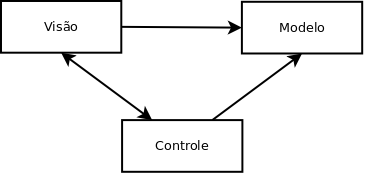
\includegraphics[width=0.5\textwidth]{fig/diagrama_mvc.png}
\caption{Arquitetura MVC}
\label{fig:diag_mvc}
\end{figure}

O modelo de acesso a dados é representado pela camada Model (ou camada de modelo). O modelo 
é um objeto que representa alguma informação sobre o domínio. É um objeto não-visual 
que contém todos os dados e comportamentos outros que não os utilizados 
pela interface \cite{Fowler:2006}.

A camada View (ou camada de visão) representa a interface da aplicação. No trabalho
em questão, ela é a parte em HTML. Esta camada não deve possuir nenhuma lógica de negócio,
detendo-se apenas à captura e exibição de dados.

A camada Controller (ou camada de controle) é a responsável por conectar as outras duas
camadas. O controlador recebe a entrada do usuário (capturado pela visão), manipula o 
modelo e faz com que a visão seja atualizada apropriadamente \cite{Fowler:2006}.

\subsubsection{ORM}
Atualmente a maioria das aplicações é desenvolvida utilizando o paradigma de programação 
orientado a objetos e um banco de dados relacional. Essas aplicações precisam carregar
dados de um banco de dados, criar objetos para representar esses dados em memória,
executar operações em cima destes objetos e depois salvar de volta as alterações no banco.

Ferramentas de mapeamento objeto-relacional (ou ORM) são frameworks que recuperam e persistem
objetos. Seu objetivo é dar suporte à complexa atividade de gerenciar conexões entre
objetos e um banco de dados relacional. A persistência fica transparente ao desenvolvedor,
já que ele não precisa se preocupar com os detalhes de implementação. A ponte entre
objetos e seus relacionamentos é realizada pela ferramenta ORM segundo a especificação 
de mapeamento dos dados \cite{springerlink}.

\subsubsection{Convention over configuration}
Frameworks de propósito geral normalmente necessitam de um ou mais arquivos de configuração
para serem utilizados. Um arquivo de configuração mapeia uma classe e um recurso (uma tabela
no banco de dados) ou um evento (uma requisição web). À medida em que a complexidade das
aplicações cresce, os arquivos de configuração também crescem, tornando-se difíceis de manter \cite{Chen}. 
Para evitar este mal desnecessário, muitos frameworks atualmente procuram seguir o modelo
de desenvolvimento de software de Convenção sobre Configuração (Convention over Configuration).
A idéia é basicamente fazer com que o desenvolvedor só precise definir aquilo que não segue 
uma convenção pré-estabelecida. 

\begin{figure}[!htbp]
\begin{minipage}[t]{0.5\linewidth}
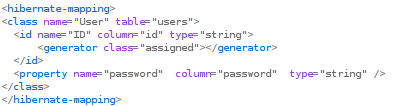
\includegraphics[scale=0.75]{fig/coc_hibernate.png}
\caption{Definição de um mapeamento no Hibernate}\label{fig:coc_hibernate}
\end{minipage} \hfill
\begin{minipage}[t]{0.3\linewidth}
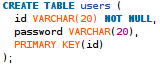
\includegraphics[scale=0.75]{fig/coc_tabela.png}
\caption{Tabela Users no banco de dados}\label{fig:coc_tabela}
\end{minipage}
\end{figure}

A Figura ~\ref{fig:coc_hibernate} apresenta um arquivo de mapeamento para Hibernate,
um framework de mapeamento objeto-relacional para Java. O código da Figura ~\ref{fig:coc_hibernate}
mapeia a classe User com a tabela Users no banco de dados. A tabela Users é descrita 
na Figura ~\ref{fig:coc_tabela} usando SQL. Os campos da classe User também são mapeados
para as colunas da tabela Users.

O ato de modificar arquivos de configuração, normalmente em XML, é tedioso e propenso
a erros. A maioria dos problemas de configuração só vai ser detectado em tempo de execução,
disparando exceções na aplicação, que tendem a diminuir o ritmo do desenvolvimento e 
consequentemente a produtividade. Mais importante ainda, uma grande parte do
mapeamento poderia ser inferido facilmente pela estrutura da tabela sem a necessidade
de configuração alguma. 

Por exemplo, pode-se estabelecer uma convenção de que:
\begin{enumerate}
\item Nomes de tabelas devem ser o nome da classe no plural.
\item As colunas na tabela devem ter nomes idênticos aos campos que a classe mapeia.
\end{enumerate}

Estas duas convenções são naturais, e, de fato, já são seguidas pela maioria dos desenvolvedores.
O padrão de convenção sobre configuração reduz a quantidade de configuração ao estabelecer
um conjunto de convenções de nomenclatura que todos os desenvolvedores devem seguir \cite{Chen}.

\subsection{SGBD}
O PostgreSQL é um SGBD (Sistema de Gerenciamento de Banco de Dados) livre, de código aberto,
bastante robusto e confiável. Derivou-se do projeto POSTGRES da universidade de Berkley, que 
iniciou-se em 1986 e foi patrocinado por instituições militares americanas como a DARPA
 (Agência de Projetos de Pesquisa Avançada para Defesa) e ARO (Departamento de Pesquisa Militar).
A linguagem de consultas SQL foi inserida quando o nome do projeta era Postgres95, tendo sido
rebatizado para o nome atual em 1996 para enfatizar a relação do SGBD com o SQL \cite{postgresql}.

Apesar do PostgreSQL ter sido escolhido para o desenvolvimento deste trabalho, outros SGBDs
podem ser utilizados em seu lugar, devido ao framework Symfony possuir um ORM que abstrai
a comunicação da aplicação com o banco de dados. Basta configurar a conexão do banco de dados
no Symfony e avisá-lo qual SGBD estará em uso que o seu ORM se encarregará de fazer a comunicação
correta com o banco de dados.

\subsection{IDE}
O NetBeans é um ambiente integrado de desenvolvimento (IDE) gratuito, também de codigo aberto e 
atualmente patrocinado pela Oracle. Originalmente suportava apenas a linguagem Java, mas atualmente
consegue trabalhar com diversas linguagem de programação, entre elas o PHP, e além disso possui plugins
que facilitam a utilização de alguns frameworks, inclusive o Symfony.

Foi escolhido para este trabalho por fornecer um bom suporte ao PHP e ao Symfony, e por possuir fácil
integração com a ferramenta de depuração Xdebug, específica para PHP.

\section{Requisitos da aplicação}

\begin{itemize}
\item[PHP] Deve ser utilizada a versão 5.2.4 ou mais recente (exceto a versão 5.2.9).
\item[Servidor] Recomenda-se a utilização do servidor Apache versão 2 ou superior, com a extensão
mod\_rewrite instalada. O projeto não foi testado com outros servidores HTTP.
\item[SGBD] Recomenda-se PostgreSQL 8.4 como SGBD por ter sido utilizado durante o desenvolvimento da aplicação, mas
de acordo com a documentação do Doctrine, o ORM do Symfony, qualquer banco de dados suportado pelo PHP através 
dos drivers PDO pode ser utilizado, já que ele utiliza PDO para se comunicar com o banco de dados.
A aplicação foi seguramente testada com MySQL Community Edition 5.5.9 e SQLite 3.7.5, podendo estes 
também serem utilizados sem prejuízo algum ao funcionamento do sistema. Para qualquer que seja o
banco escolhido, o driver PDO deve estar instalado e configurado no PHP.
\item[E-mail] É necessária uma conta de email em um servidor que aceite conexões externas via SMTP para
o envio das mensagens eletrônicas. Alternativamente pode-se utilizar o Sendmail, caso este esteja
configurado no servidor, ou deixar a cargo da função mail do PHP. Recomenda-se configurar um
servidor SMTP, especialmente pela facilidade de configuração deste se comparado ao Sendmail. Não 
é recomendado utilizar a função mail do PHP, pois os emails enviados tendem a ser identificados
como spam em muitos servidores de email.


\end{itemize}



\section{Arquitetura}
\subsection{Diagrama de classes}

\chapter{Utilização do sistema}
\label{cha:utilizacao}

Neste capítulo descrevemos inicialmente a utilização do sistema. A descrição tende
a ser sucinta, visto que a ferramenta é bastante simples e as telas são auto-explicativas.
Posteriormente, descrevemos os principais passos para a instalação e configuração
do sistema no servidor web.

\section{Utilização do sistema}
O TCC-Manager consiste de vários módulos, que possuem comportamentos diferentes dependendo do 
tipo de usuário que está autenticado no sistema. São 4 (quatro) perfis possíveis:
\begin{itemize}
\item[Administrador] Adminstrador do sistema. Cabe a este perfil cadastrar alunos e professores.
Ele também tem acesso somente-leitura às propostas e defesas.
\item[Estudante] Possui acesso somente a manutenção de seus próprios projetos.
\item[Professor] Possui acesso às propostas e solicitações de defesa de seus orientandos.
\item[Comissão] Possui acesso a todas as propostas e solicitações de defesa do sistema.
\end{itemize}

Devido a essas diferenças de perfis, dividiremos a utilização do sistema de acordo com cada um.

\subsection{Telas em comum entre todos os perfis}
A tela de acesso ao sistema (Figura ~\ref{fig:tela_login}) e a tela de acesso negado (Figura ~\ref{fig:tela_acesso_negado}) são as mesmas para todos os perfis.
Na tela de acesso ao sistema (Figura ~\ref{fig:tela_login}), o campo login espera receber o nome de usuário
para todos os perfis exceto para estudantes, que devem digitar a sua matrícula.

A tela de acesso negado (Figura ~\ref{fig:tela_acesso_negado}) é exibida quando um usuário tenta acessar uma tela de outro perfil, sem
ter a permissão necessária para isso.

\begin{figure}[htbp]
\centering

\includegraphics[width=1\textwidth]{fig/telas/login.png}
\caption{Tela de acesso ao sistema}
\label{fig:tela_login}
\end{figure}

\begin{figure}[htbp]
\centering
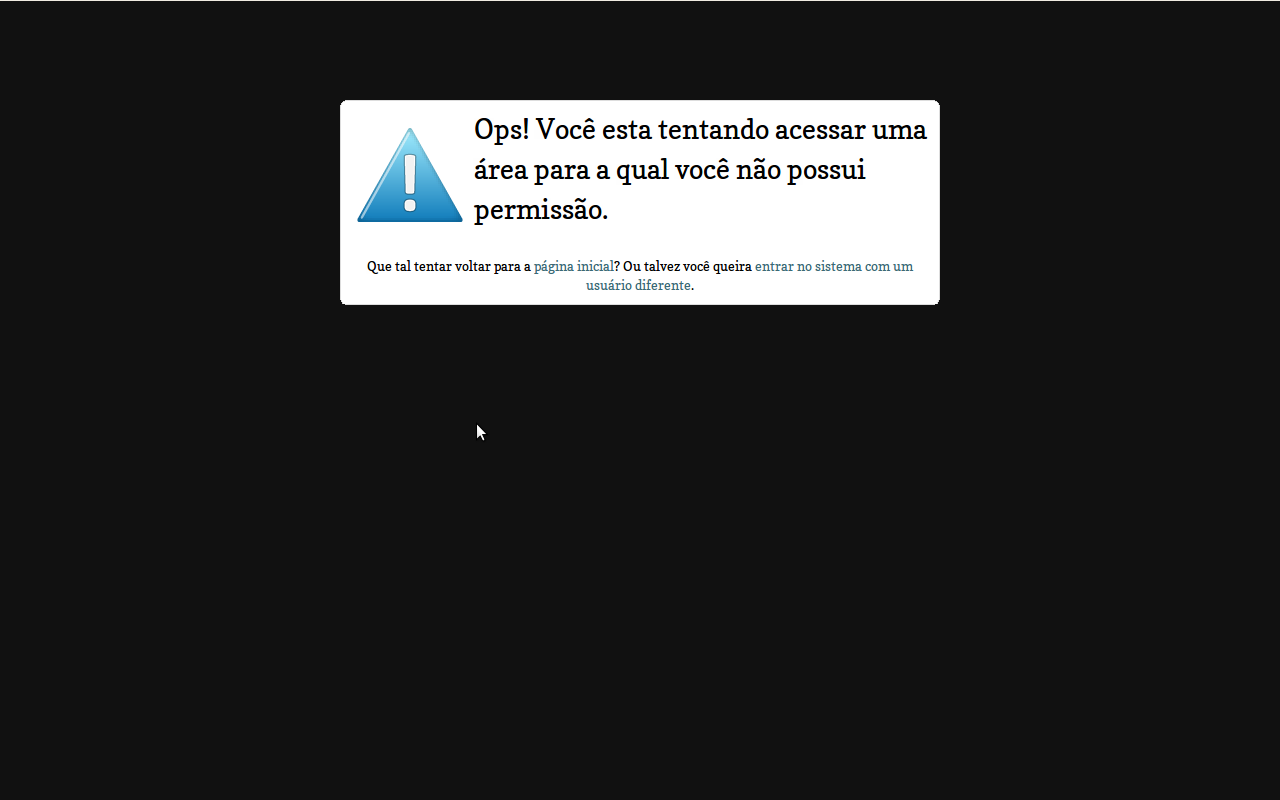
\includegraphics[width=1\textwidth]{fig/telas/acesso_negado.png}
\caption{Tela de acesso negado}
\label{fig:tela_acesso_negado}
\end{figure}


\subsection{Perfil de administrador}
O perfil do administrador consiste basicamente dos cadastros do sistema. A seguir veremos as
telas de cadastro de professores, alunos e semestres. Em seguida vemos que este perfil também
pode visualizar quais propostas e defesas estão cadastradas no banco de dados e pode 
consultar relatórios.

\begin{figure}[htbp]
\centering
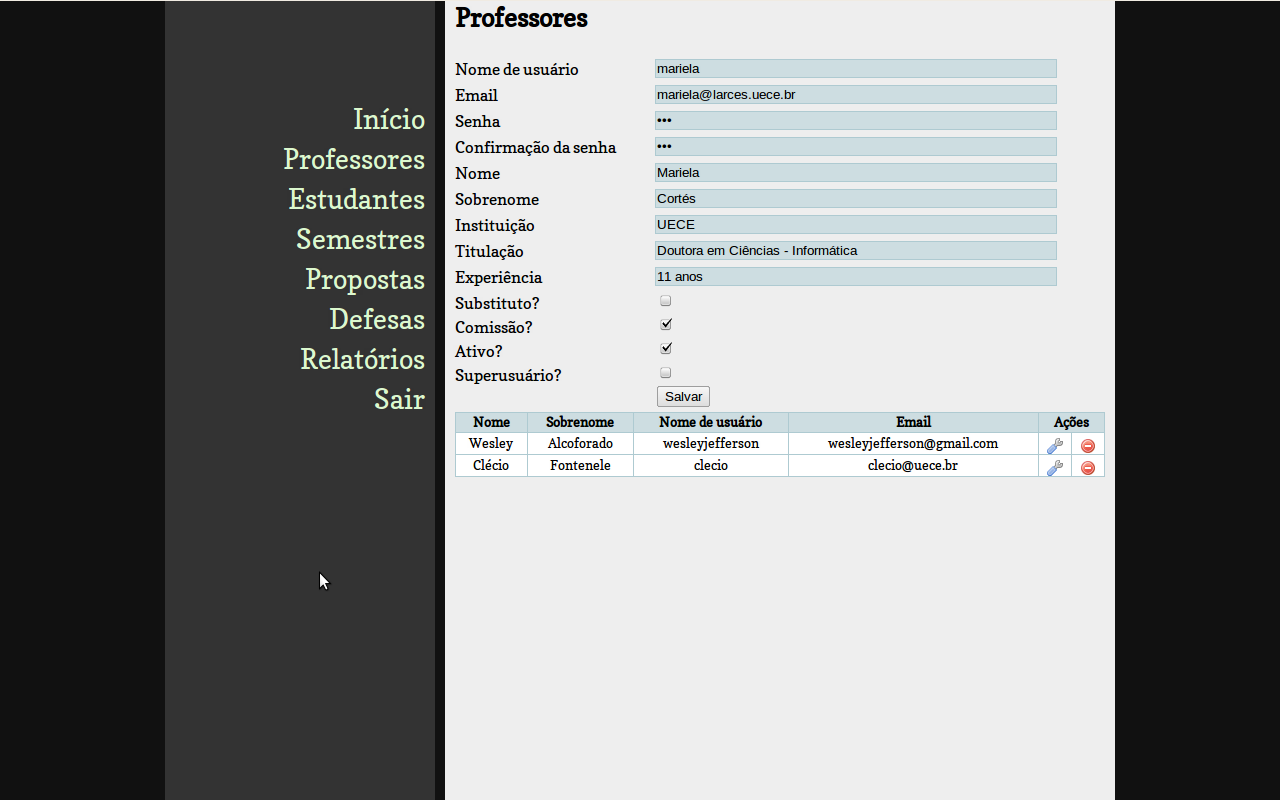
\includegraphics[width=1\textwidth]{fig/telas/administrador/crud_professor_insercao.png}
\caption{Tela de cadastro de professores}
\label{fig:crud_professor_insercao}
\end{figure}

\begin{figure}[htbp]
\centering
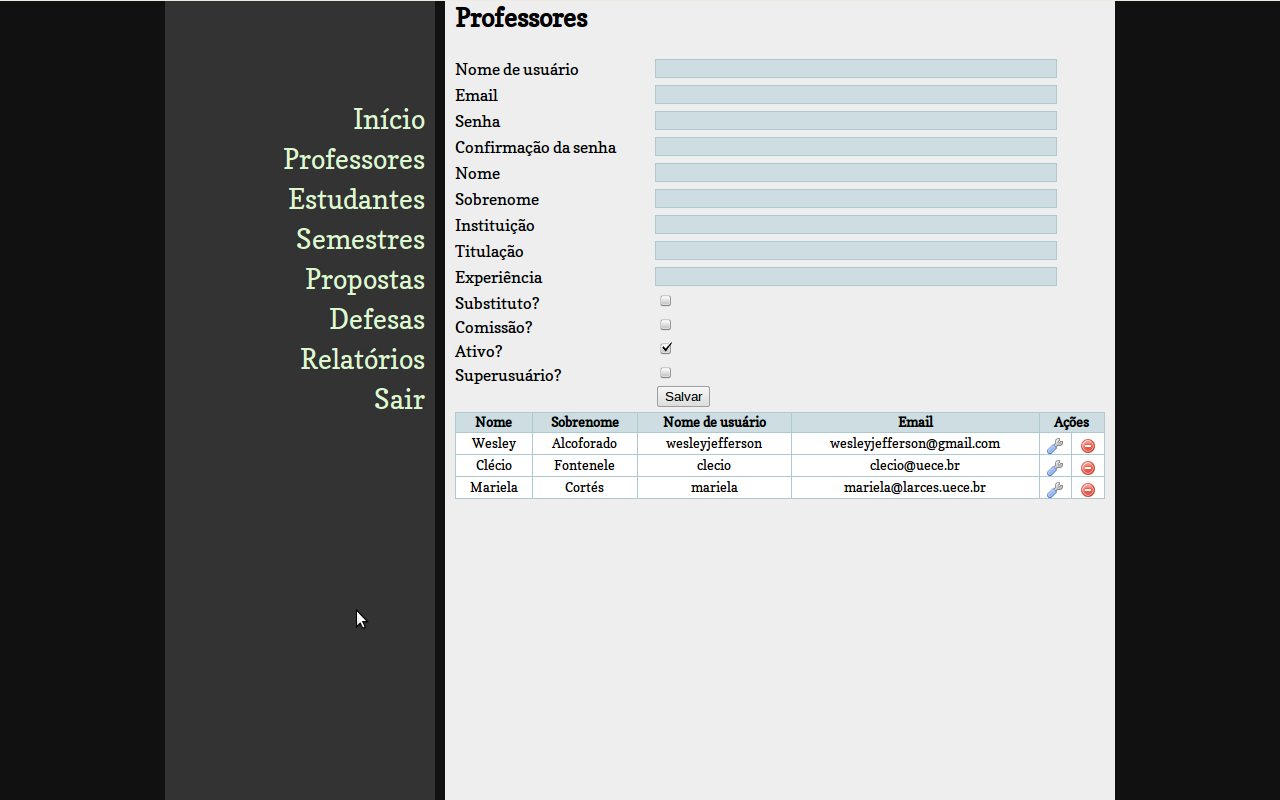
\includegraphics[width=1\textwidth]{fig/telas/administrador/crud_professor_listagem_pos_insercao.png}
\caption{Tela de cadastro de professores após a inserção de um professor}
\label{fig:crud_professor_listagem_pos_insercao}
\end{figure}

\begin{figure}[htbp]
\centering
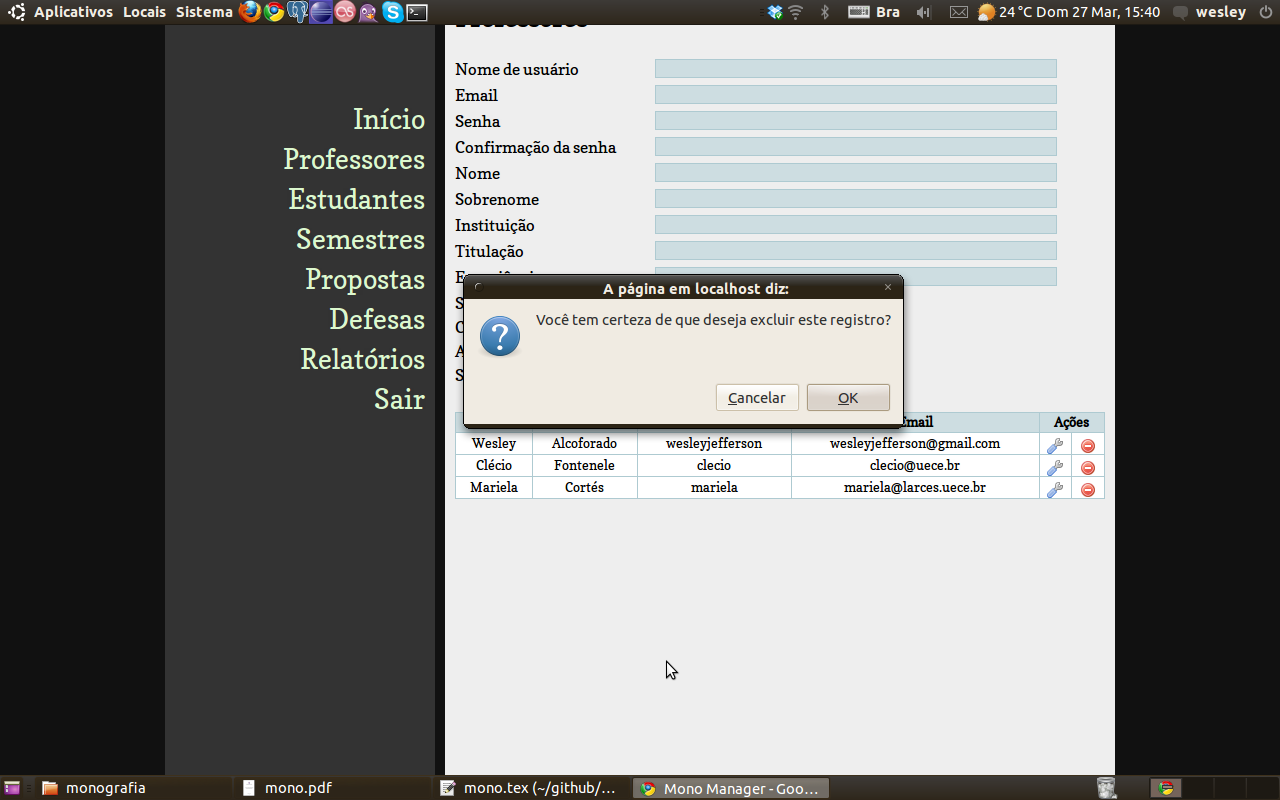
\includegraphics[width=1\textwidth]{fig/telas/administrador/crud_professor_remocao.png}
\caption{Confirmação de remoção de um professor}
\label{fig:crud_professor_remocao}
\end{figure}

Na Figura ~\ref{fig:crud_professor_insercao} mostra a tela de cadastro de professores, que
é acessada ao clicar na opção Professor no menu do sistema. Podemos ver que na tela
já se encontram disponíveis o formulário de edição e a listagem de todos os professores cadastrados 
no sistema. Na coluna Ações, na listagem de professores, estão disponíveis as ações de edição
e remoção de registro. A Figura ~\ref{fig:crud_professor_insercao} exibe o formulário sendo preenchido
para a inserção de um novo professor, ao passo que a Figura ~\ref{fig:crud_professor_listagem_pos_insercao}
exibe a listagem atualizada após a inserção de um novo professor no sistema. Se o administrador 
clicar no ícone de remoção de registro, uma janela de confirmação é exibida para que
o administrador confirme seu desejo de remoção do registro, visto que esta ação não pode
ser revertida. Este processo pode ser visualizado na Figura ~\ref{fig:crud_professor_remocao}.

\begin{figure}[htbp]
\centering
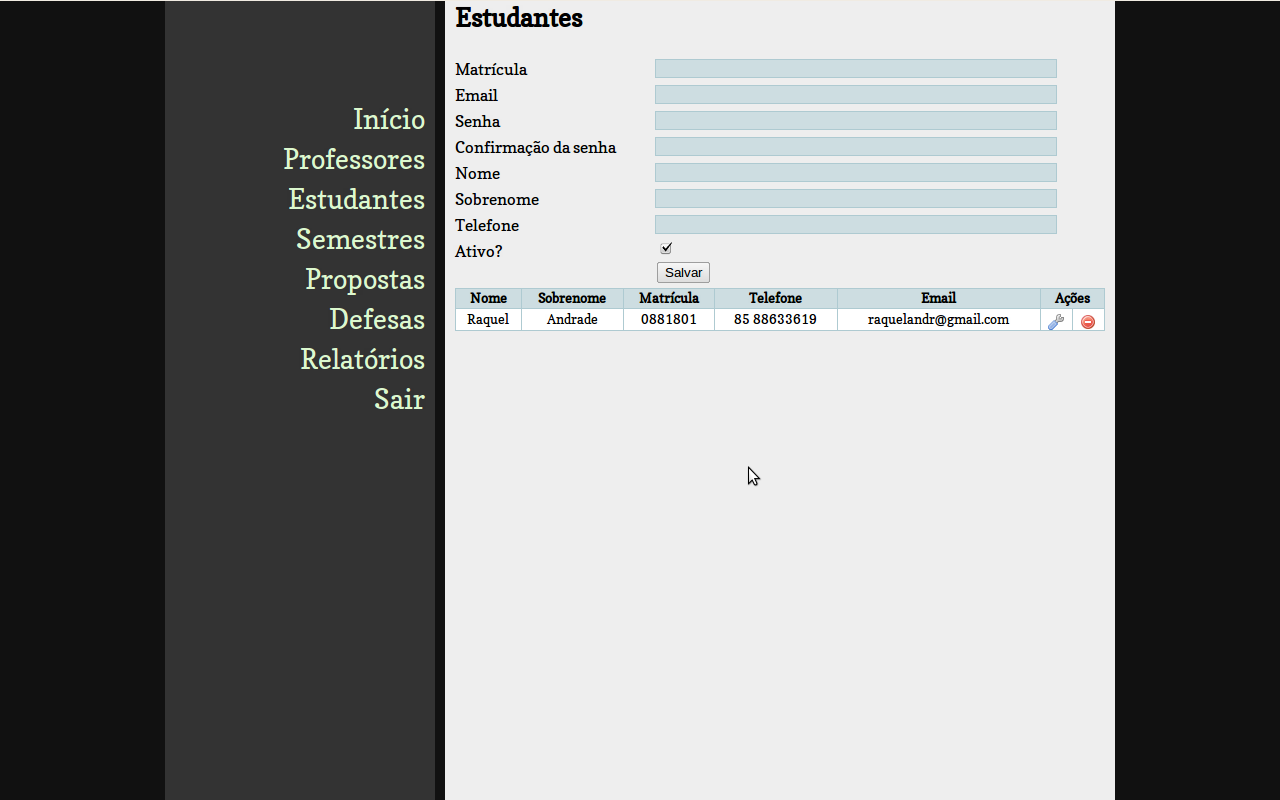
\includegraphics[width=1\textwidth]{fig/telas/administrador/crud_estudante.png}
\caption{Tela de cadastro de estudantes}
\label{fig:crud_estudante}
\end{figure}

A Figura ~\ref{fig:crud_estudante} exibe a tela de cadastro de estudantes. O mecanismo de funcionamento
desta é exatamente igual ao de cadastro de professores, portanto não há necessidade de mais detalhes.

\begin{figure}[htbp]
\centering
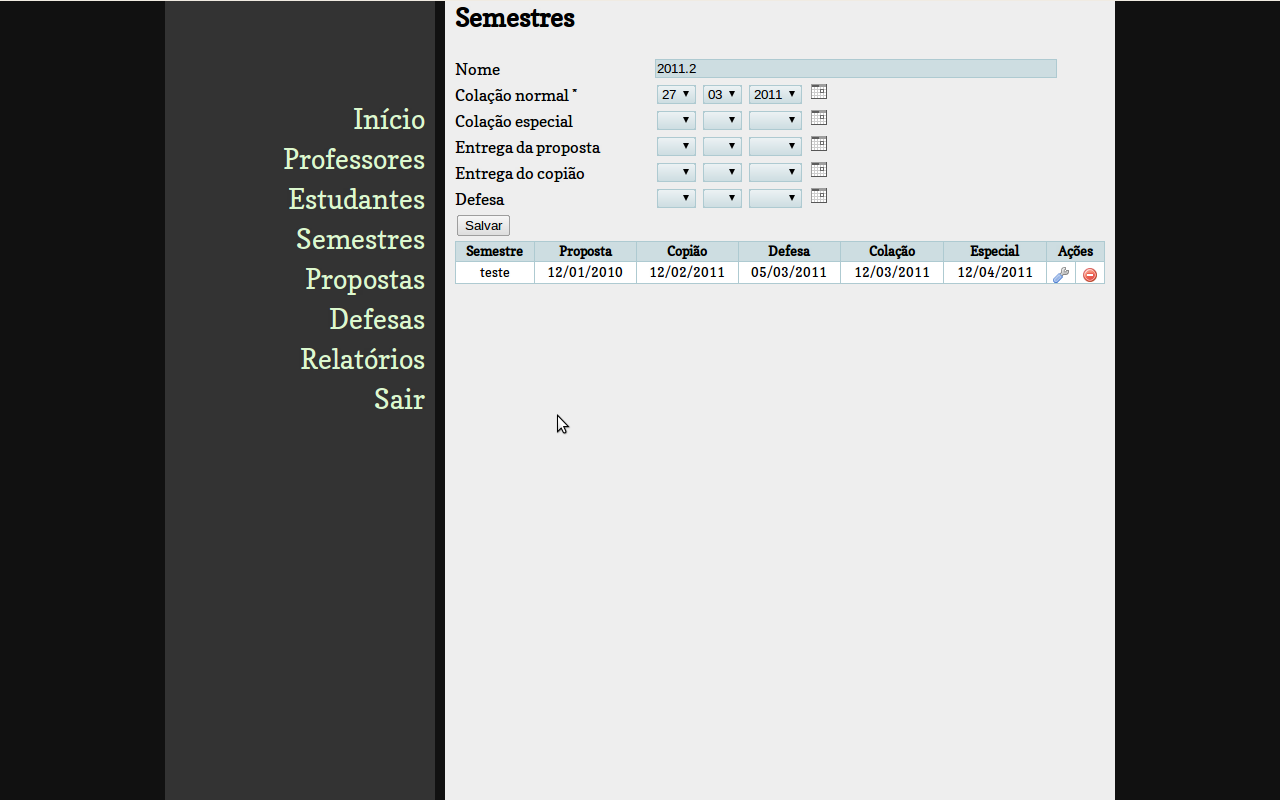
\includegraphics[width=1\textwidth]{fig/telas/administrador/crud_semestre.png}
\caption{Tela de cadastro de semestres}
\label{fig:crud_semestre}
\end{figure}

\begin{figure}[htbp]
\centering
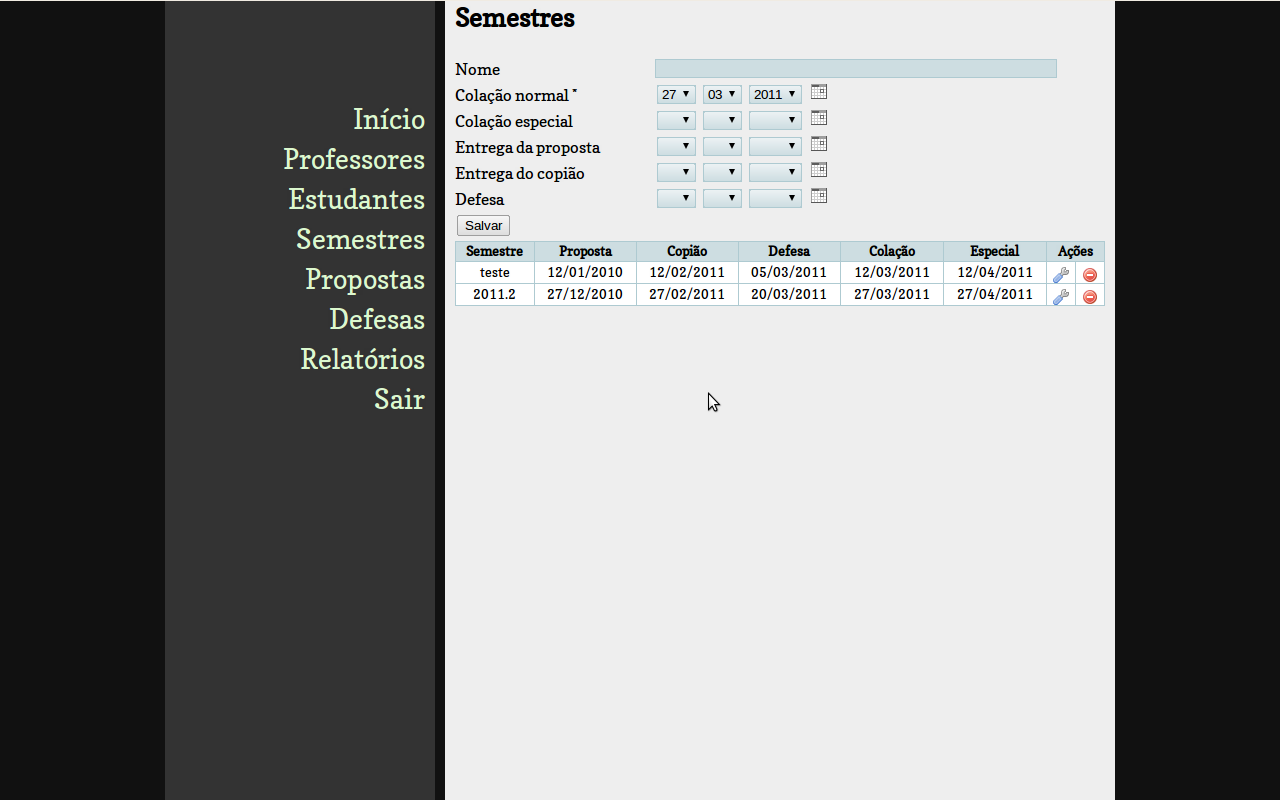
\includegraphics[width=1\textwidth]{fig/telas/administrador/crud_semestre_calculo_datas.png}
\caption{Tela de cadastro de semestres após o cadastro de um novo item}
\label{fig:crud_semestre_calculo_datas}
\end{figure}

A Figura ~\ref{fig:crud_semestre} mostra a tela de cadastro de semestres. Esta possui um funcionamento
muito parecido com o cadastro de professores e estudantes, porém possui uma particularidade que 
convém explicitar. O único campo obrigatório é a data de colação normal. A partir da informação desta
data, pode-se inferir todas as outras. O cálculo é feito a partir das informações estabelecidas
no regulamento da universidade, que pode ser conferido nas Seções ~\ref{sec:proposta} e ~\ref{sec:defesa}.
A Figura ~\ref{fig:crud_semestre_calculo_datas} exibe o item inserido no banco de dados com as
datas calculadas a partir da data de colação normal. Se por algum motivo as datas forem diferentes,
o administrador pode informá-las separadamente. O sistema só tenta calcular aquelas que não foram
informadas.

\begin{figure}[htbp]
\centering
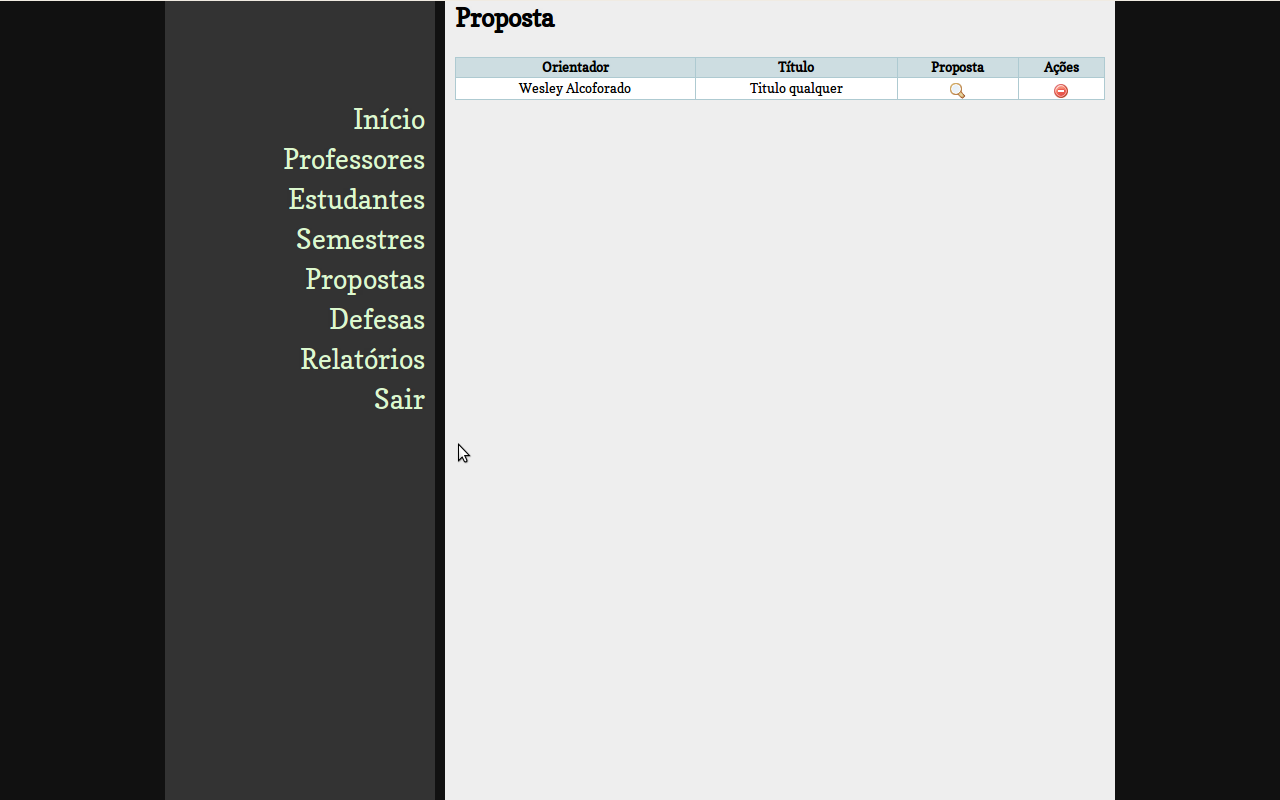
\includegraphics[width=1\textwidth]{fig/telas/administrador/propostas.png}
\caption{Tela de visualização de propostas no perfil do administrador}
\label{fig:propostas}
\end{figure}

\begin{figure}[htbp]
\centering
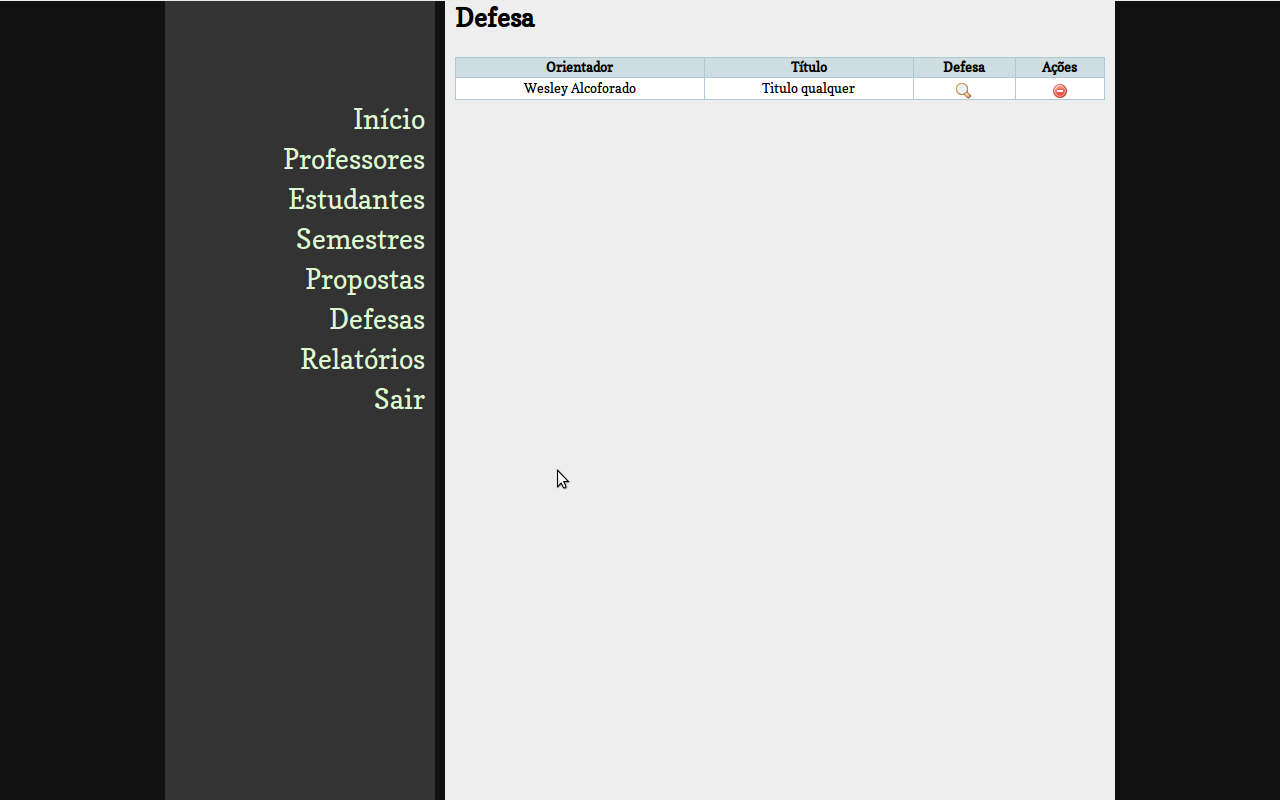
\includegraphics[width=1\textwidth]{fig/telas/administrador/defesas.png}
\caption{Tela de visualização de defesas no perfil do administrador}
\label{fig:defesas}
\end{figure}

\begin{figure}[htbp]
\centering
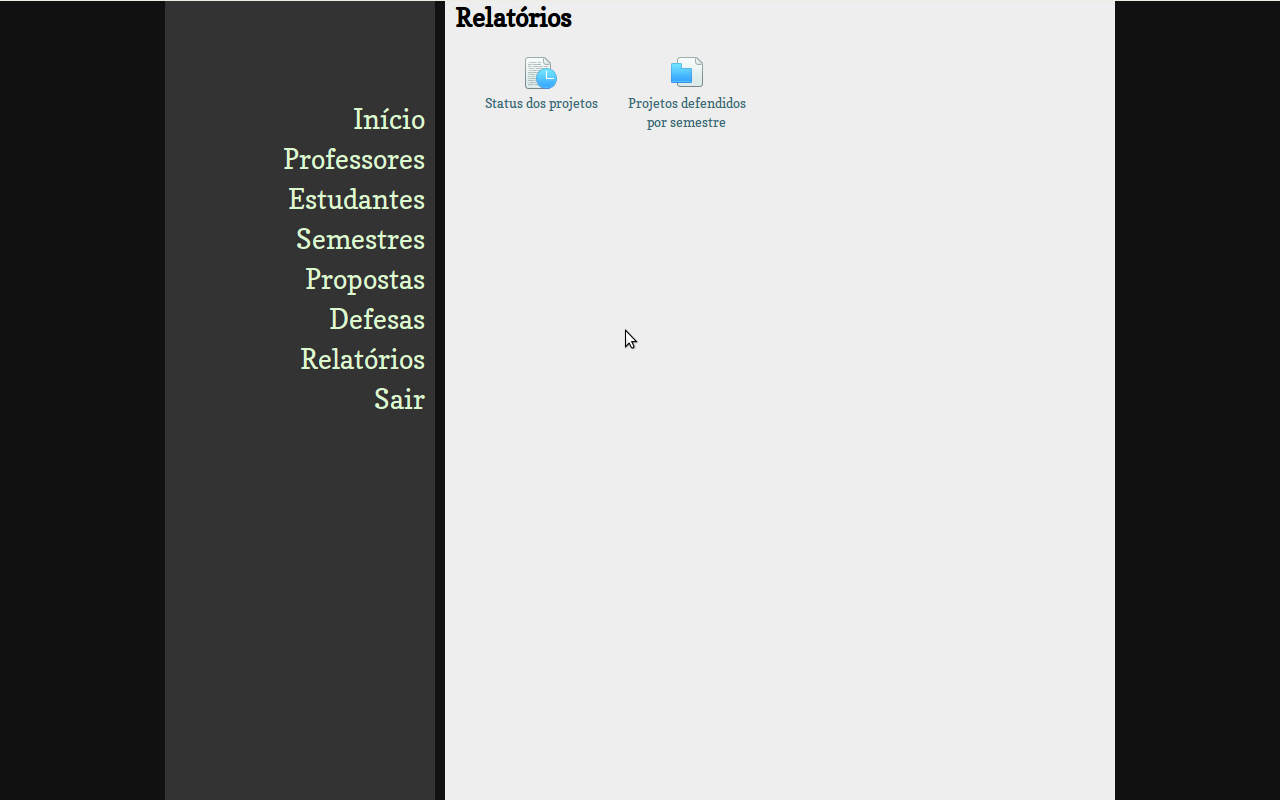
\includegraphics[width=1\textwidth]{fig/telas/administrador/relatorios.png}
\caption{Tela de consulta de relatórios}
\label{fig:relatorios}
\end{figure}

A Figura ~\ref{fig:propostas} exibe a tela de visualização de propostas e a Figura ~\ref{fig:defesas}
exibe a tela de visualização de defesas no perfil do administardor. Ambas possuem um ícone em formato
de lupa que permite visualizar a proposta do projeto ou o copião (no caso de uma solicitação de defesa), e
possuem um ícone para remover o registro do banco de dados. A Figura ~\ref{fig:relatorios} exibe a tela
de consulta de relatórios, que é compartilhada entre os perfis de administrador e comissão.

\subsection{Perfil de estudante}
O estudante só precisa se preocupar com o desenvolvimento do seu próprio projeto, por isso, o único
módulo que ele precisa ter acesso é o de projetos. A Figura ~\ref{fig:aluno_01_projeto_novo} exibe
o formulário de projetos sendo preenchido pelo estudante, onde ele só precisa informar o nome do
seu projeto e quem são seus orientadores. A Figura ~\ref{fig:aluno_02_projeto_cadastrado} exibe como fica
a listagem de projetos após a inserção do novo item. Podemos notar que quando o projeto é cadastrado, seu 
status indica que a proposta está pendente. A Figura ~\ref{fig:aluno_03_anexo_proposta} exibe a tela de anexo
de propostas, que pode ser acessada pelo ícone em formato de clipe na coluna Proposta. Após a anexação
da proposta (Figura ~\ref{fig:aluno_04_proposta_anexada}), um email é enviado ao orientador, informando-o
que um de seus alunos acabou de anexar uma proposta e que sua aprovação é necessária. O aluno
deve aguardar que o orientador e a comissão aprovem sua proposta para iniciar o desenvolvimento do
trabalho. Quando isso acontecer, o estudante deverá receber um email notificando a novidade.
As Figuras ~\ref{fig:aluno_05_proposta_aprovada_orientador} e ~\ref{fig:aluno_06_proposta_aprovada_comissao}
demonstram as modificações do status do projeto à medida que o orientador e a comissão avaliam 
a sua proposta.

A partir da tela da Figura ~\ref{fig:aluno_06_proposta_aprovada_comissao}, o ícone em formato de apresentação
de slides fica disponível para o estudante, significando que ele pode submeter uma solicitação de defesa. Ao
clicar no ícone, a tela da Figura ~\ref{fig:aluno_07_submetendo_defesa} é carregada, solicitando ao
estudante os itens necessários para a solicitação da defesa, como o documento do copião.

As Figuras ~\ref{fig:aluno_08_defesa_nao_analisada}, ~\ref{fig:aluno_09_defesa_analisada_professor}, 
~\ref{fig:aluno_10_defesa_analisada_comissao} e ~\ref{fig:aluno_11_projeto_defendido} mostram 
respectivamente a evolução do status do projeto à medida em que o estudante solicita
a defesa, o orientador a aprova, a comissão a aprova e a comissão identifica que a defesa foi efetivamente concluida.


\begin{figure}[htbp]
\centering
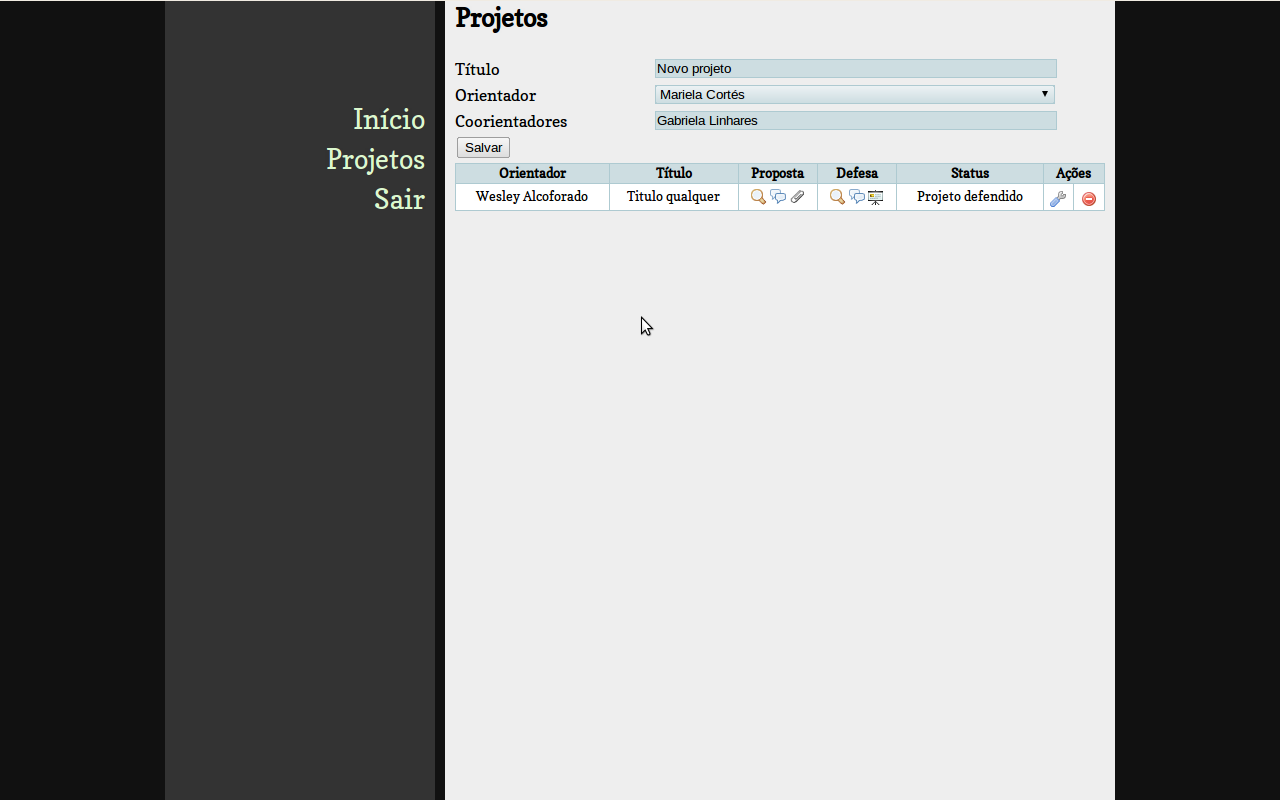
\includegraphics[width=1\textwidth]{fig/telas/processo/aluno_01_projeto_novo.png}
\caption{Tela de cadastro de projetos}
\label{fig:aluno_01_projeto_novo}
\end{figure}

\begin{figure}[htbp]
\centering
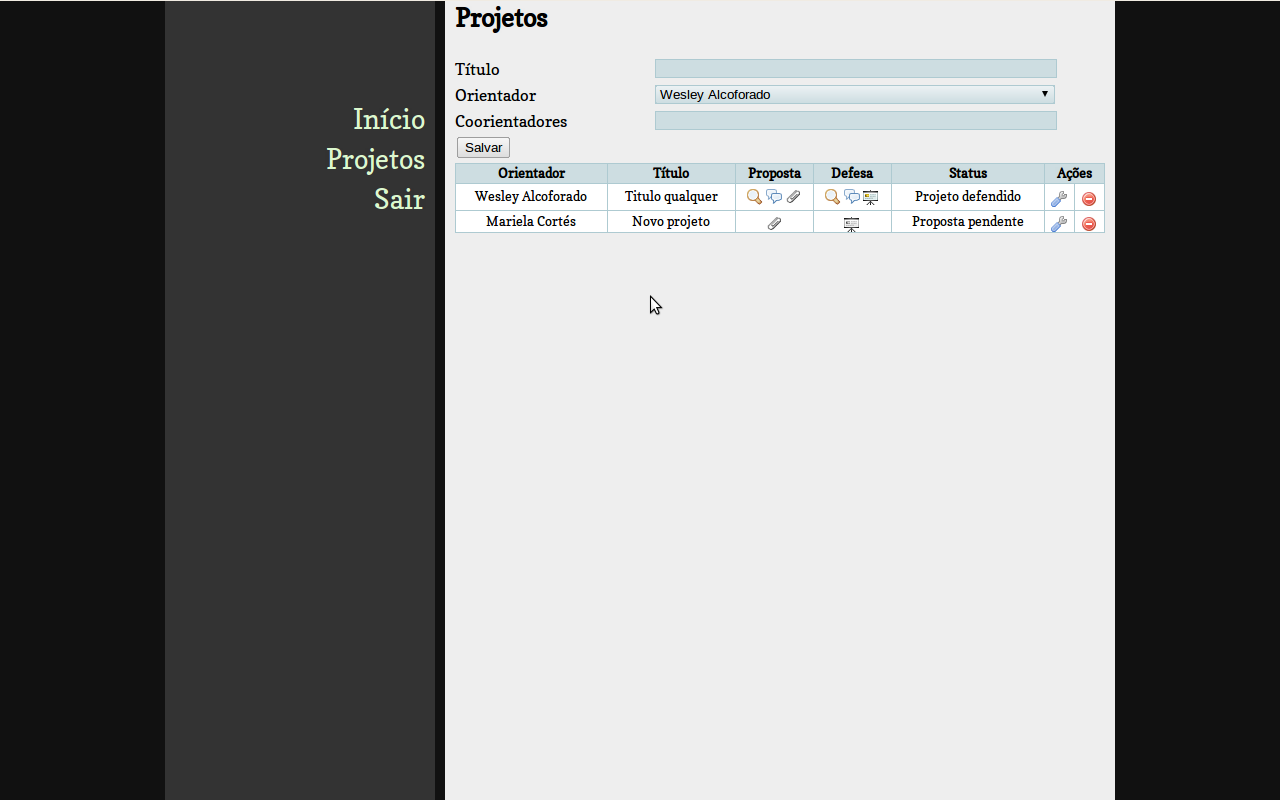
\includegraphics[width=1\textwidth]{fig/telas/processo/aluno_02_projeto_cadastrado.png}
\caption{Tela de cadastro de projetos após a inserção de novo item}
\label{fig:aluno_02_projeto_cadastrado}
\end{figure}

\begin{figure}[htbp]
\centering
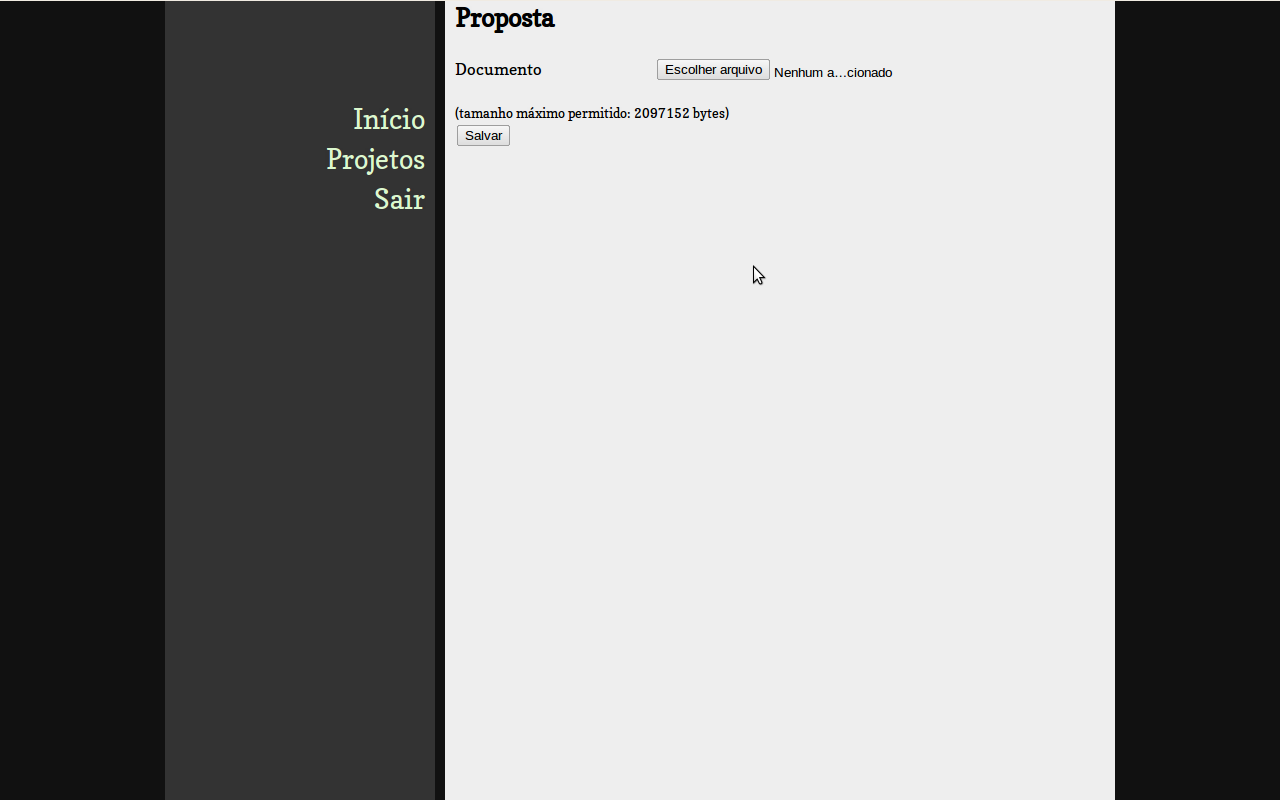
\includegraphics[width=1\textwidth]{fig/telas/processo/aluno_03_anexo_proposta.png}
\caption{Tela de anexo de propostas}
\label{fig:aluno_03_anexo_proposta}
\end{figure}

\begin{figure}[htbp]
\centering
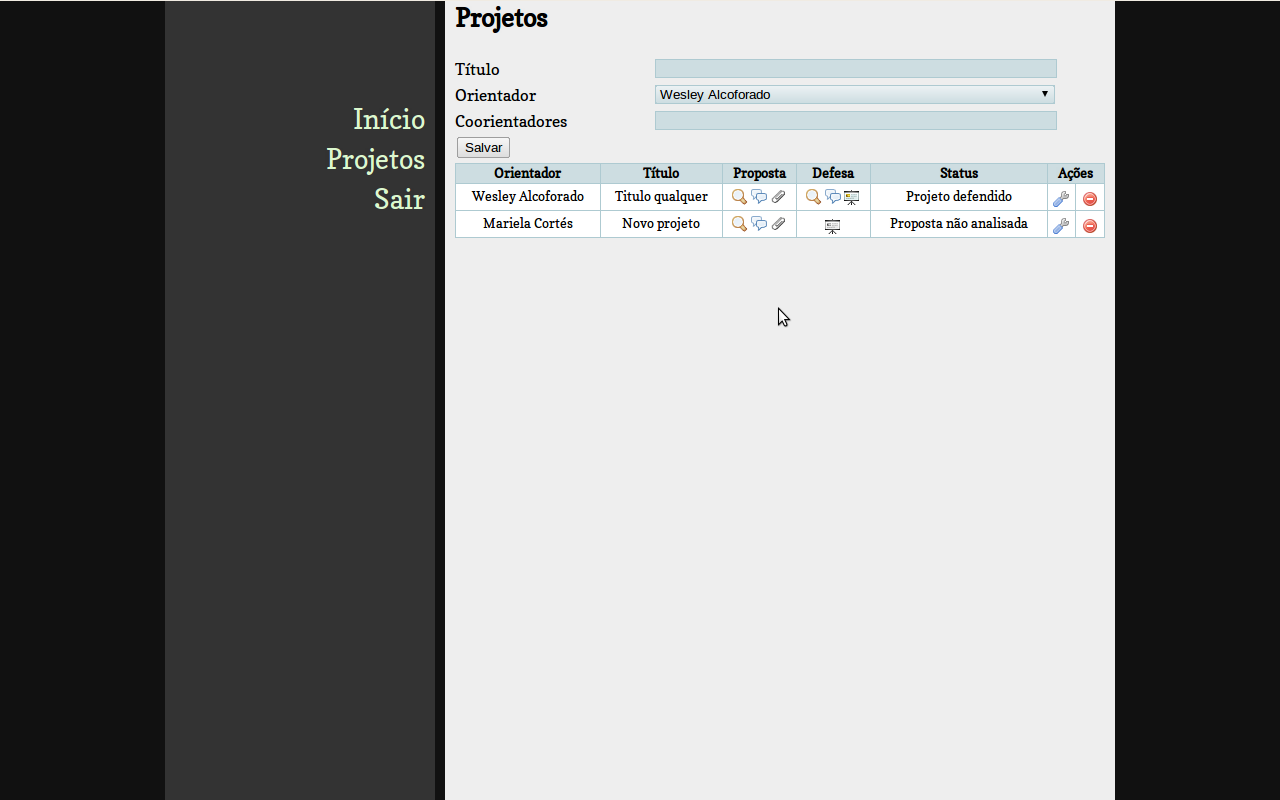
\includegraphics[width=1\textwidth]{fig/telas/processo/aluno_04_proposta_anexada.png}
\caption{Tela de cadastro de projetos após a anexação de uma proposta}
\label{fig:aluno_04_proposta_anexada}
\end{figure}

\begin{figure}[htbp]
\centering
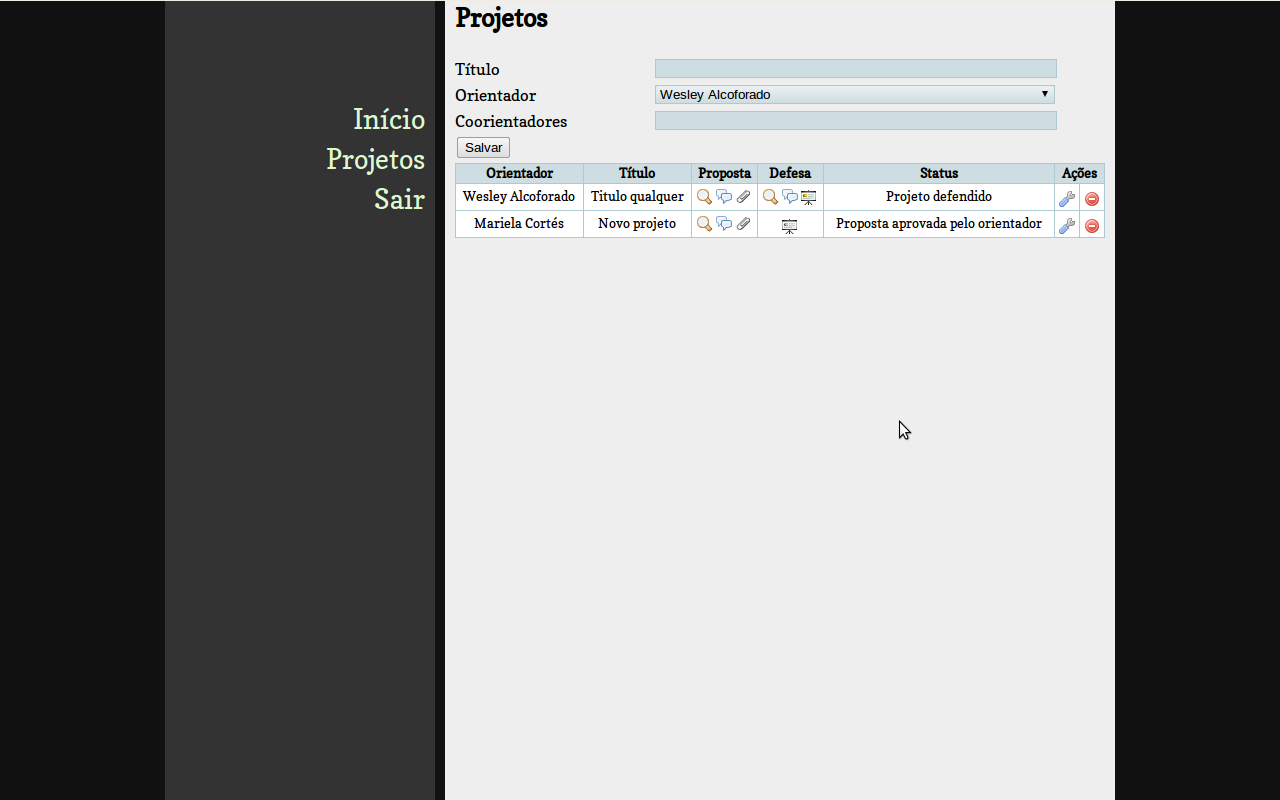
\includegraphics[width=1\textwidth]{fig/telas/processo/aluno_05_proposta_aprovada_orientador.png}
\caption{Tela de cadastro de projetos após a aprovação do orientador}
\label{fig:aluno_05_proposta_aprovada_orientador}
\end{figure}

\begin{figure}[htbp]
\centering
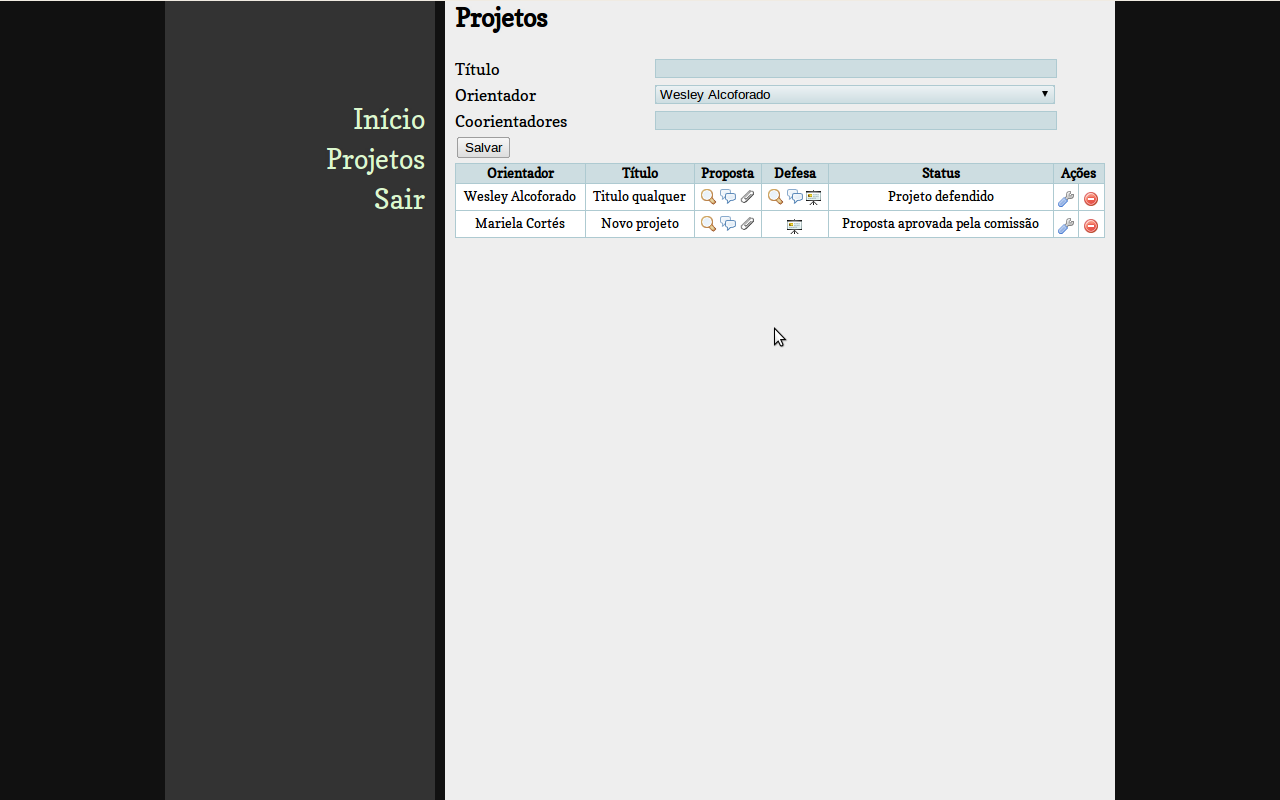
\includegraphics[width=1\textwidth]{fig/telas/processo/aluno_06_proposta_aprovada_comissao.png}
\caption{Tela de cadastro de projetos após a aprovação da comissão}
\label{fig:aluno_06_proposta_aprovada_comissao}
\end{figure}

\begin{figure}[htbp]
\centering
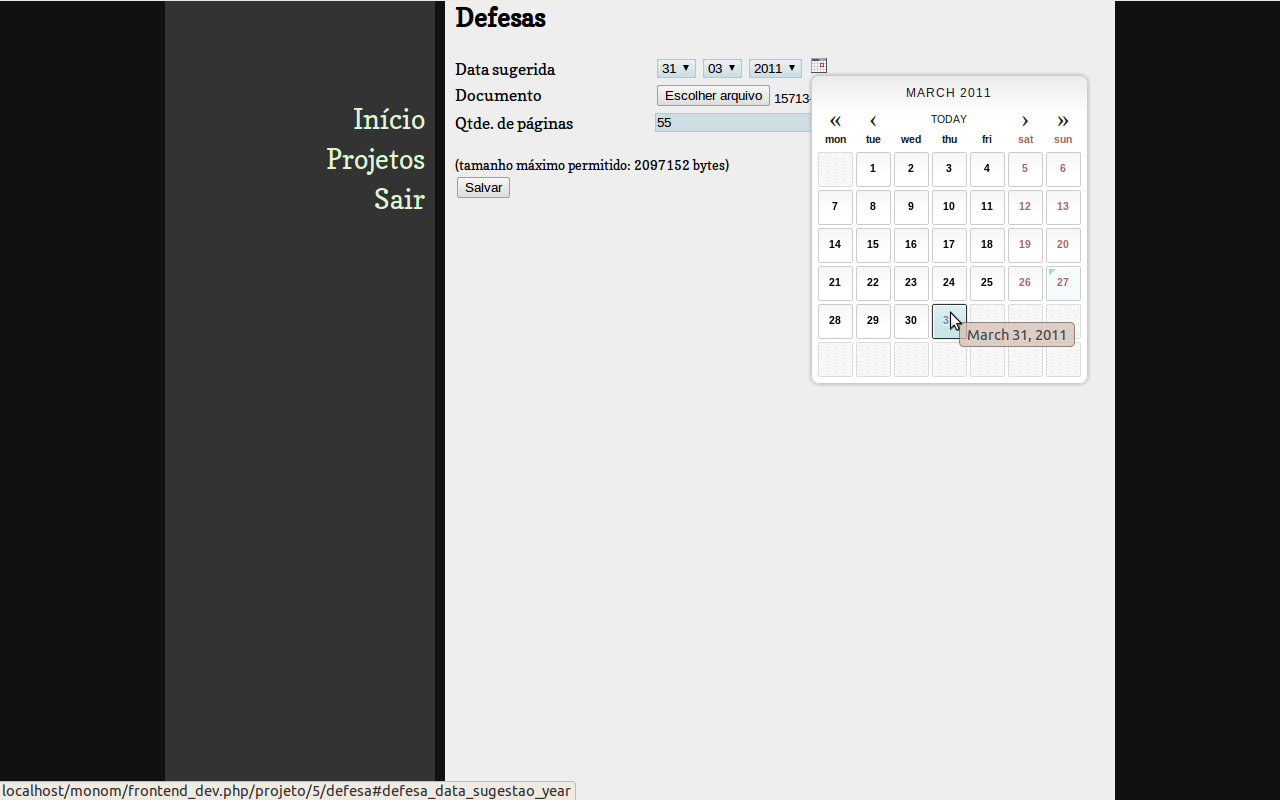
\includegraphics[width=1\textwidth]{fig/telas/processo/aluno_07_submetendo_defesa.png}
\caption{Tela de solicitação de defesa}
\label{fig:aluno_07_submetendo_defesa}
\end{figure}

\begin{figure}[htbp]
\centering
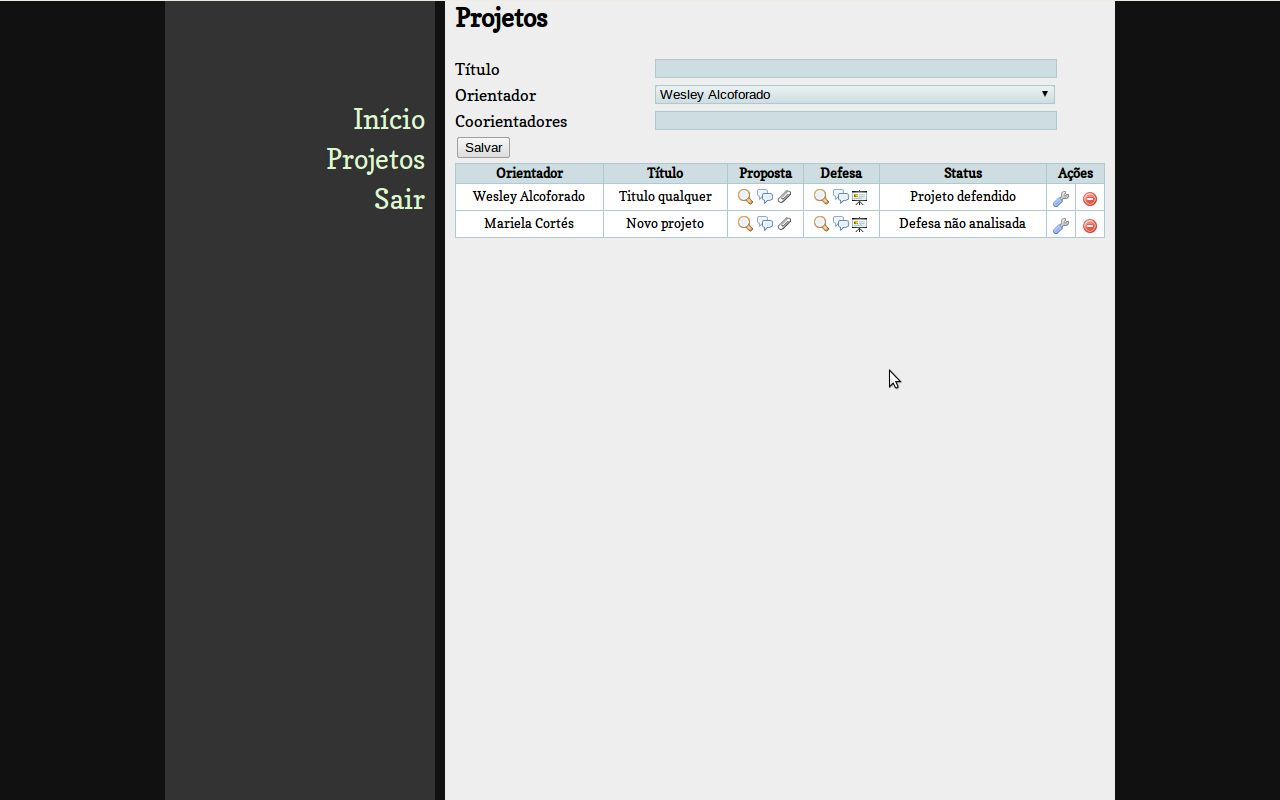
\includegraphics[width=1\textwidth]{fig/telas/processo/aluno_08_defesa_nao_analisada.png}
\caption{Tela de cadastro de projetos após a solicitação de defesa}
\label{fig:aluno_08_defesa_nao_analisada}
\end{figure}

\begin{figure}[htbp]
\centering
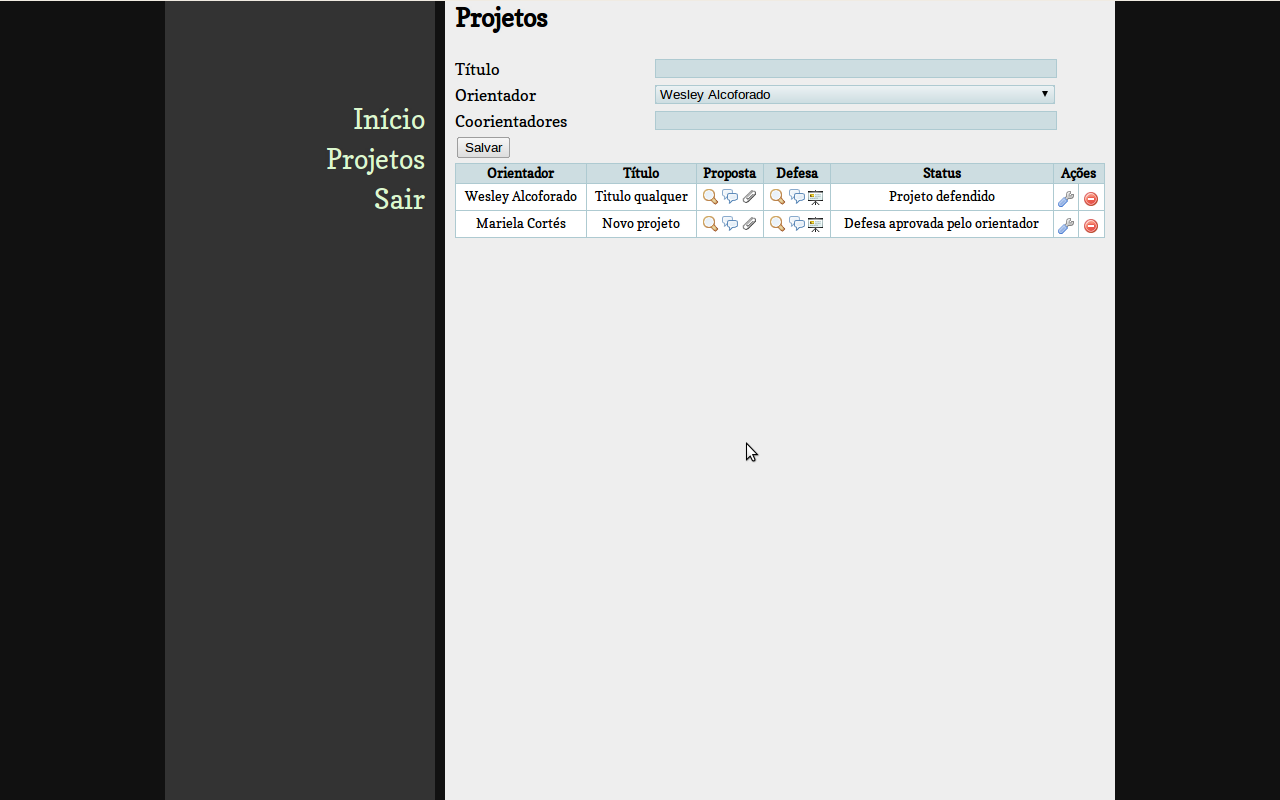
\includegraphics[width=1\textwidth]{fig/telas/processo/aluno_09_defesa_analisada_professor.png}
\caption{Tela de cadastro de projetos após a aprovação do orientador}
\label{fig:aluno_09_defesa_analisada_professor}
\end{figure}

\begin{figure}[htbp]
\centering
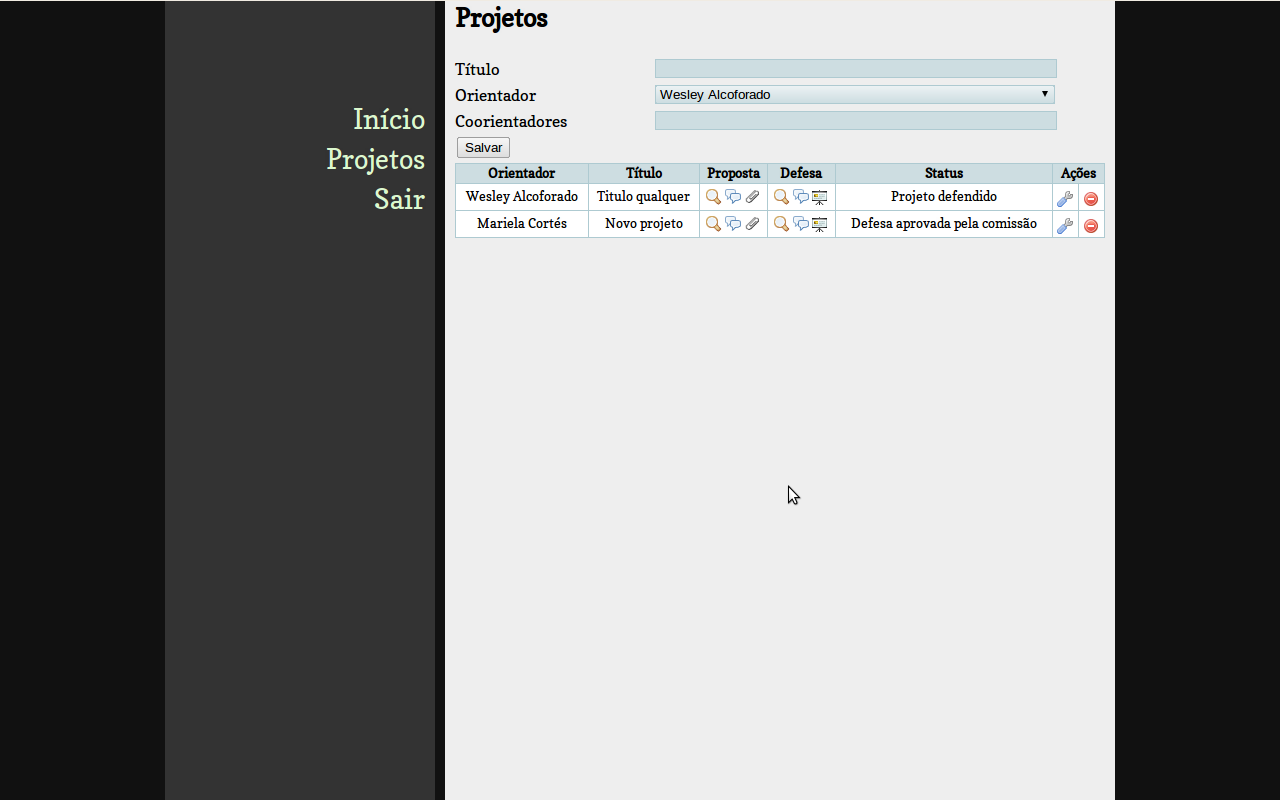
\includegraphics[width=1\textwidth]{fig/telas/processo/aluno_10_defesa_analisada_comissao.png}
\caption{Tela de cadastro de projetos após a aprovação da comissão}
\label{fig:aluno_10_defesa_analisada_comissao}
\end{figure}

\begin{figure}[htbp]
\centering
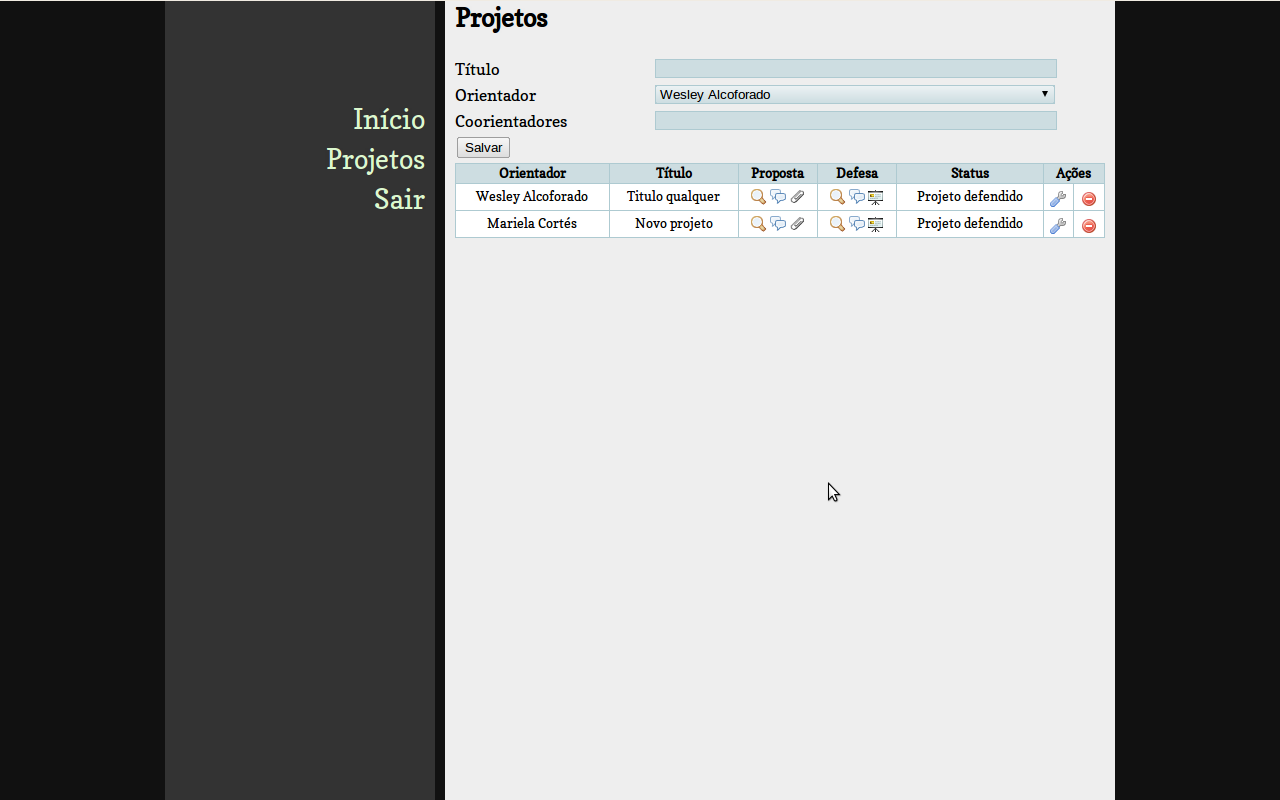
\includegraphics[width=1\textwidth]{fig/telas/processo/aluno_11_projeto_defendido.png}
\caption{Tela de cadastro de projetos após a comissão ter indicado que a defesa foi concluida}
\label{fig:aluno_11_projeto_defendido}
\end{figure}

\subsection{Perfil de professor (orientador)}
O orientador possui acesso aos projetos de seus orientandos, e deve dar o seu aval para quaisquer 
submissões que o estudante envie para a comissão de projeto final.

A Figura ~\ref{fig:professor_01_aprovacao proposta} exibe a tela de listagem de propostas
enviadas pelos orientandos. Propostas ainda não avaliadas pelo professor aparecem com dois ícones
de polegar para cima e polegar para baixo, que indicam que o professor aprova ou não a proposta, respectivamente.
Se o professor clicar no ícone em formato de lupa, ele pode visualizar o documento associado ao pedido.

A Figura ~\ref{fig:professor_02_prosta_sendo_aprovada} mostra o momento em que o professor
clica na opção de aprovar a proposta e a Figura ~\ref{fig:professor_03_proposta_aprovada} o momento
seguinte a esta ação.

Para o perfil de professor, o módulo de Defesas é completamente idêntico ao módulo de propostas, o que
podemos perceber pela Figura ~\ref{fig:professor_04_avaliando_defesa}.

\begin{figure}[htbp]
\centering
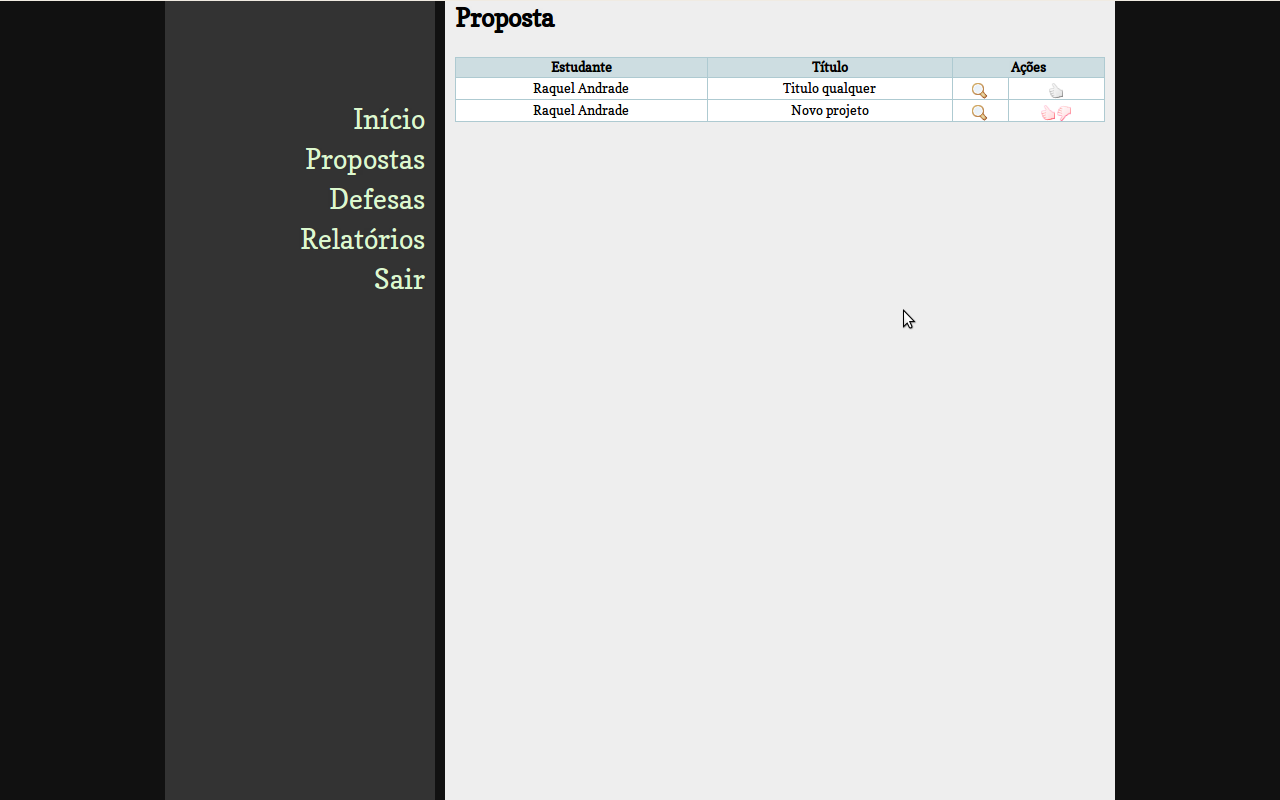
\includegraphics[width=1\textwidth]{fig/telas/processo/professor_01_aprovacao proposta.png}
\caption{Tela de listagem de propostas submetidas pelos orientandos}
\label{fig:professor_01_aprovacao proposta}
\end{figure}

\begin{figure}[htbp]
\centering
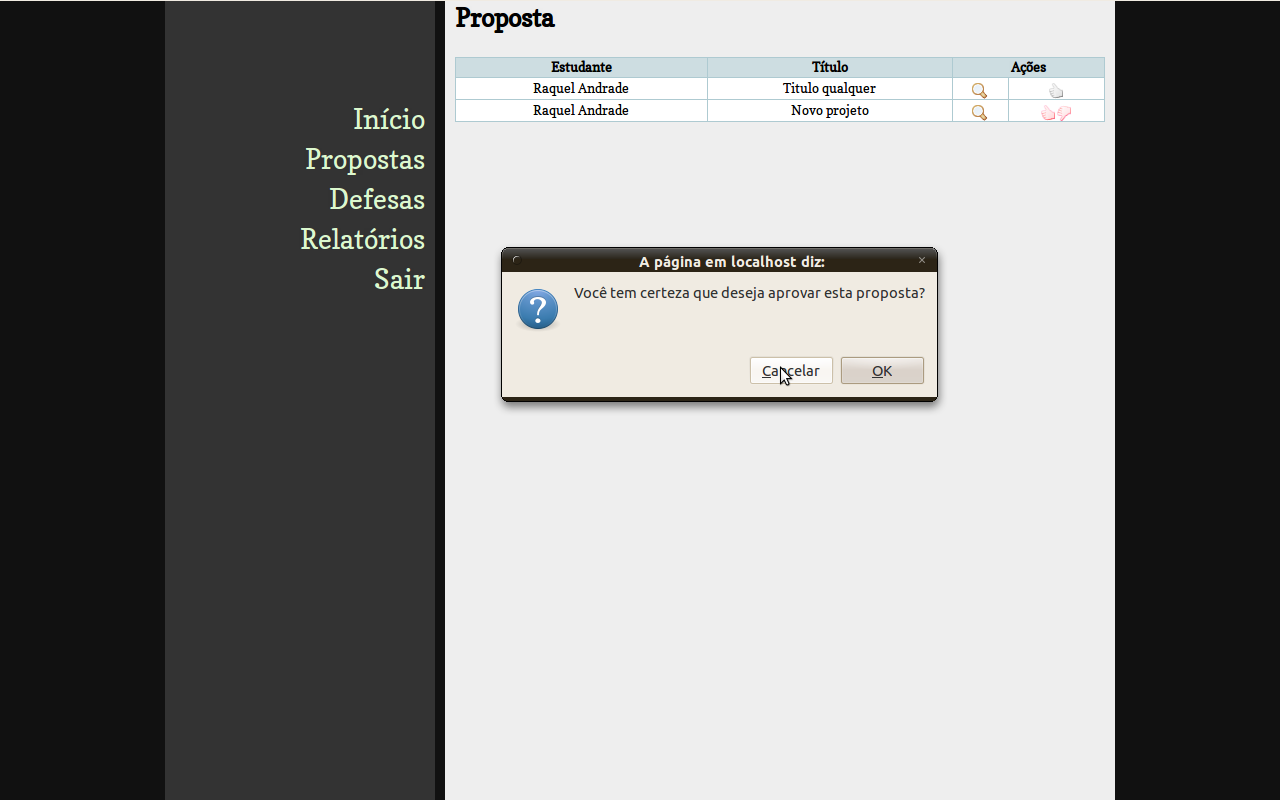
\includegraphics[width=1\textwidth]{fig/telas/processo/professor_02_prosta_sendo_aprovada.png}
\caption{Proposta sendo aprovada pelo orientador}
\label{fig:professor_02_prosta_sendo_aprovada}
\end{figure}

\begin{figure}[htbp]
\centering
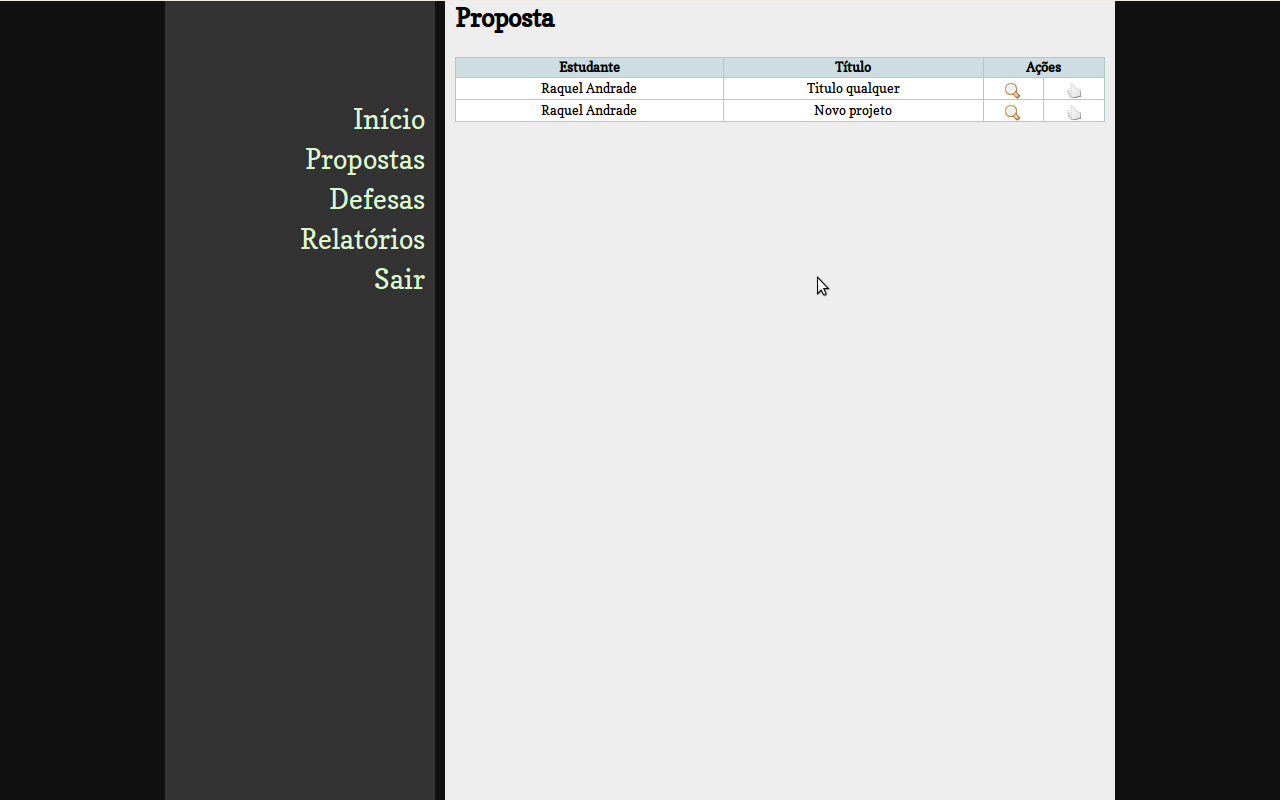
\includegraphics[width=1\textwidth]{fig/telas/processo/professor_03_proposta_aprovada.png}
\caption{Tela de listagem de propostas após o orientador ter aprovado uma proposta}
\label{fig:professor_03_proposta_aprovada}
\end{figure}

\begin{figure}[htbp]
\centering
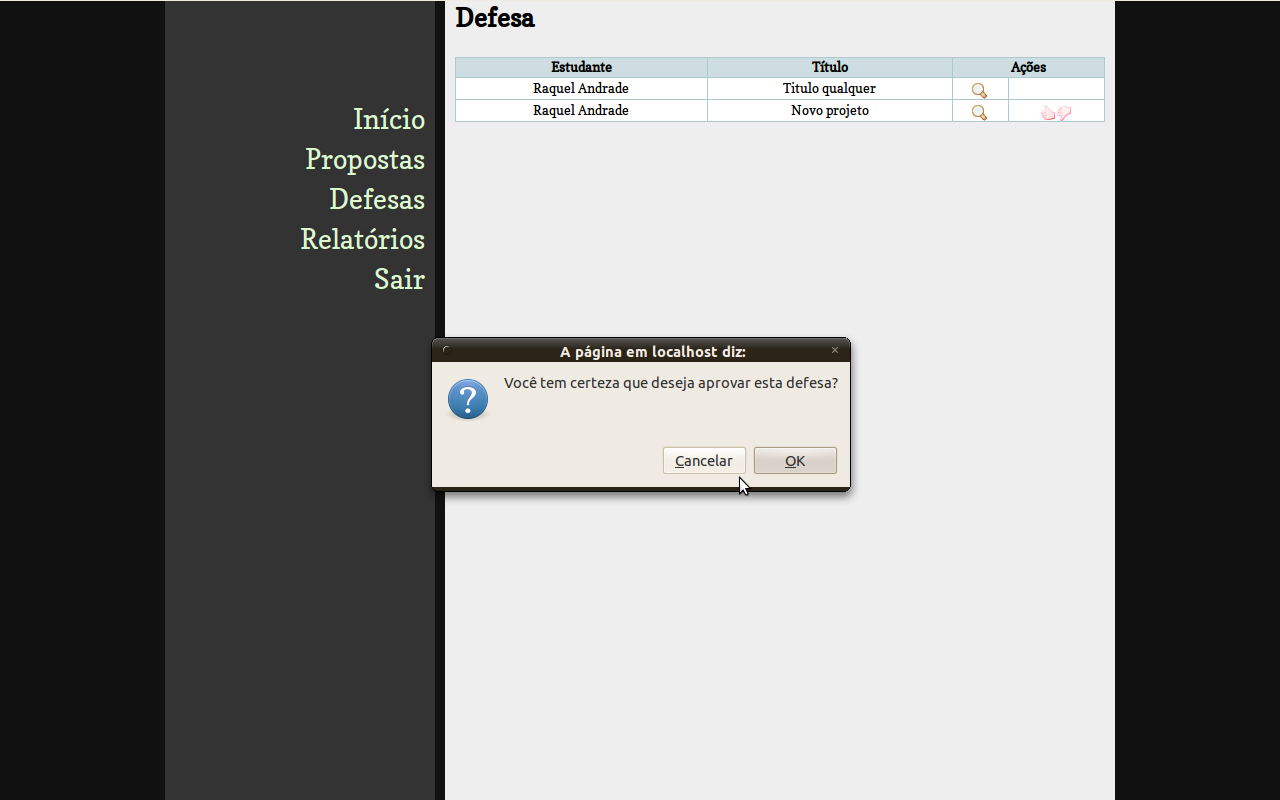
\includegraphics[width=1\textwidth]{fig/telas/processo/professor_04_avaliando_defesa.png}
\caption{Tela de listagem de requisições de defesa submetidas pelos orientandos}
\label{fig:professor_04_avaliando_defesa}
\end{figure}

\subsection{Perfil de comissão}
A comissão precisa dar o parecer final em qualquer submissão feito pelo estudante. É ela quem
decide se uma proposta de projeto pode ser desenvolvida ou não, da mesma forma que é ela quem
decide se o estudante já pode defender seu projeto.

A Figura ~\ref{fig:comissao_01_propostas} exibe a tela de listagem de propostas e uma coluna de
ações. Na primeira subcoluna, há um ícone em formato de lupa que permite à comissão visualizar
o documento da proposta anexada. O segundo ícone, em formato de balões de conversação permite
a um integrante da comissão saber quais foram os comentários feitos pelos outros integrantes sobre
a proposta em questão. O último ícone assume o formato de martelo de decisão quando a proposta
ainda não foi analisada e assume o formato de polegar para cima ou para baixo dependendo da 
avaliação final. Ao clicar no ícone do martelo, a tela da Figura ~\ref{fig:comissao_02_proposta_sendo_avaliada}
é exibida, permitindo ao integrante da comissão dar seu parecer e fornecer um comentário opcional
sobre a proposta. Uma tela de confirmação é exibida quando o integrante seleciona as opções Aprovar
ou Desaprovar, como pode ser observado na mesma figura.

A Figura ~\ref{fig:comissao_03_proposta_avaliada} exibe o status da listagem após a aprovação da
proposta e a Figura ~\ref{fig:comissao_04_comentarios} exibe a tela de comentários, que surge
após o integrante da comissão clicar no ícone em formato de balões de conversação. 

Para a avaliação das solicitações de defesa, o esquema é idêntico ao das propostas, como pode
ser observado na Figura ~\ref{fig:comissao_05_aprovando_defesa}. Existe uma pequena diferença
no ícone do martelo de decisão após a comissão aprovar a solicitação de defesa, como pode ser visto
na Figura ~\ref{fig:comissao_06_marcando_projeto_como_defendido}: o ícone é substituido por um
marcador verde, que deve ser clicado para que a comissão possa confirmar que o estudante
efetivamente defendeu o TCC e todo o seu processo foi concluido. Após a marcação deste ícone,
ele fica cinza e desabilitado.

\begin{figure}[htbp]
\centering
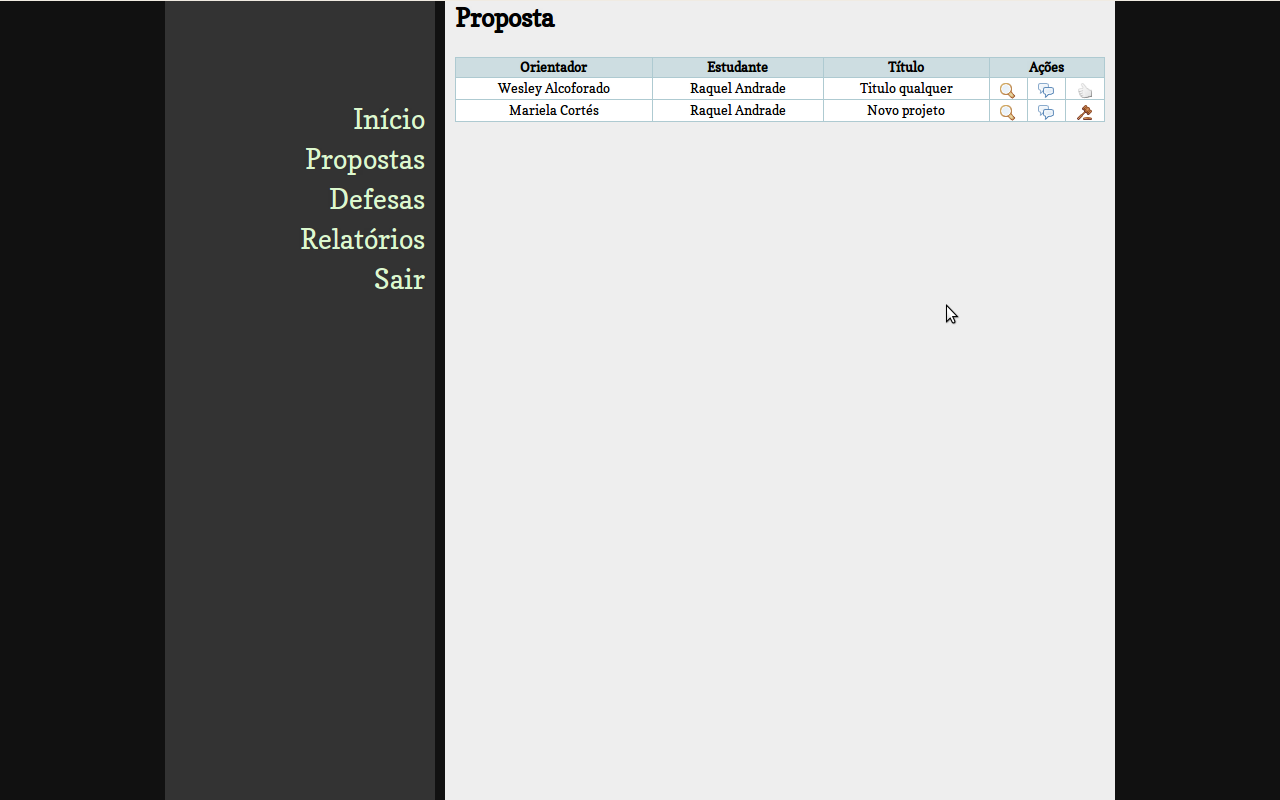
\includegraphics[width=1\textwidth]{fig/telas/processo/comissao_01_propostas.png}
\caption{Tela de listagem de propostas no perfil da comissão}
\label{fig:comissao_01_propostas}
\end{figure}

\begin{figure}[htbp]
\centering
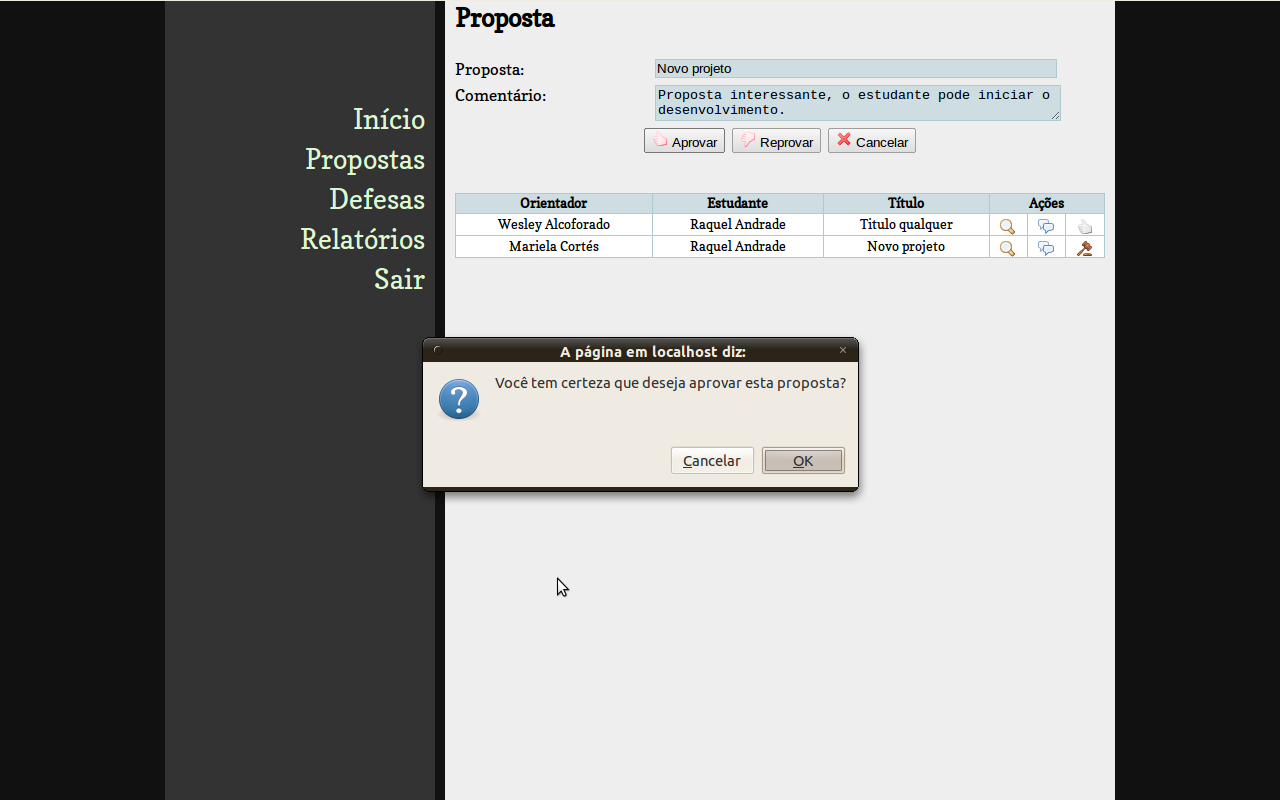
\includegraphics[width=1\textwidth]{fig/telas/processo/comissao_02_proposta_sendo_avaliada.png}
\caption{Proposta sendo avaliada pela comissão}
\label{fig:comissao_02_proposta_sendo_avaliada}
\end{figure}

\begin{figure}[htbp]
\centering
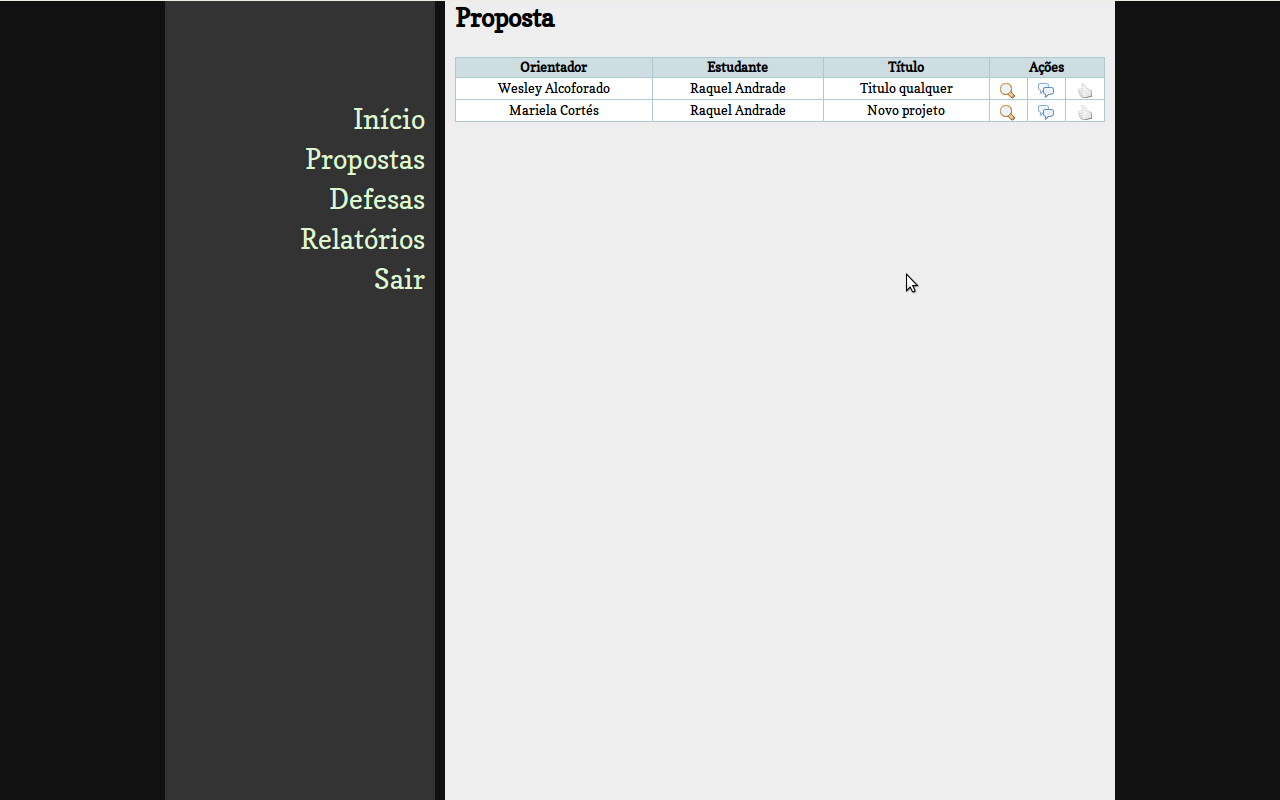
\includegraphics[width=1\textwidth]{fig/telas/processo/comissao_03_proposta_avaliada.png}
\caption{Tela de listagem de propostas após a comissão ter avaliado positivamente uma proposta}
\label{fig:comissao_03_proposta_avaliada}
\end{figure}

\begin{figure}[htbp]
\centering
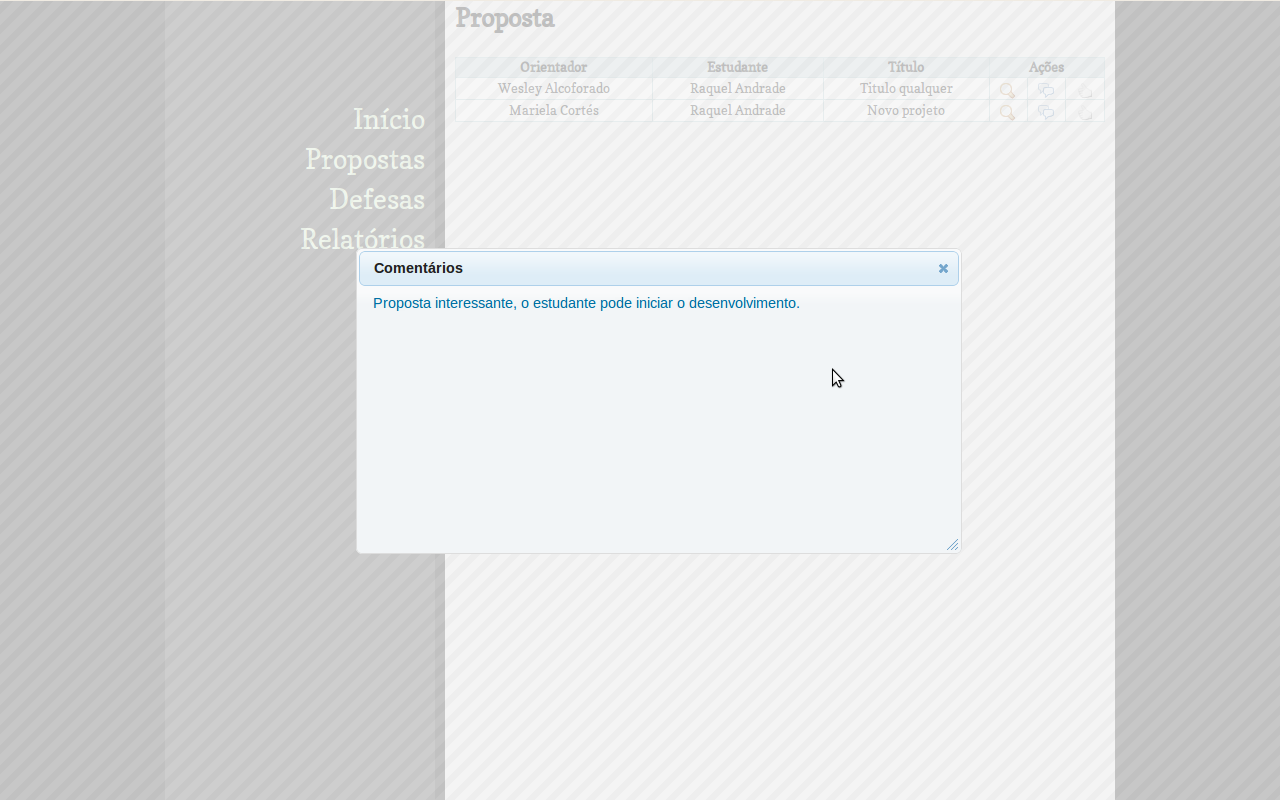
\includegraphics[width=1\textwidth]{fig/telas/processo/comissao_04_comentarios.png}
\caption{Tela de listagem de requisições de defesa submetidas pelos orientandos}
\label{fig:comissao_04_comentarios}
\end{figure}

\begin{figure}[htbp]
\centering
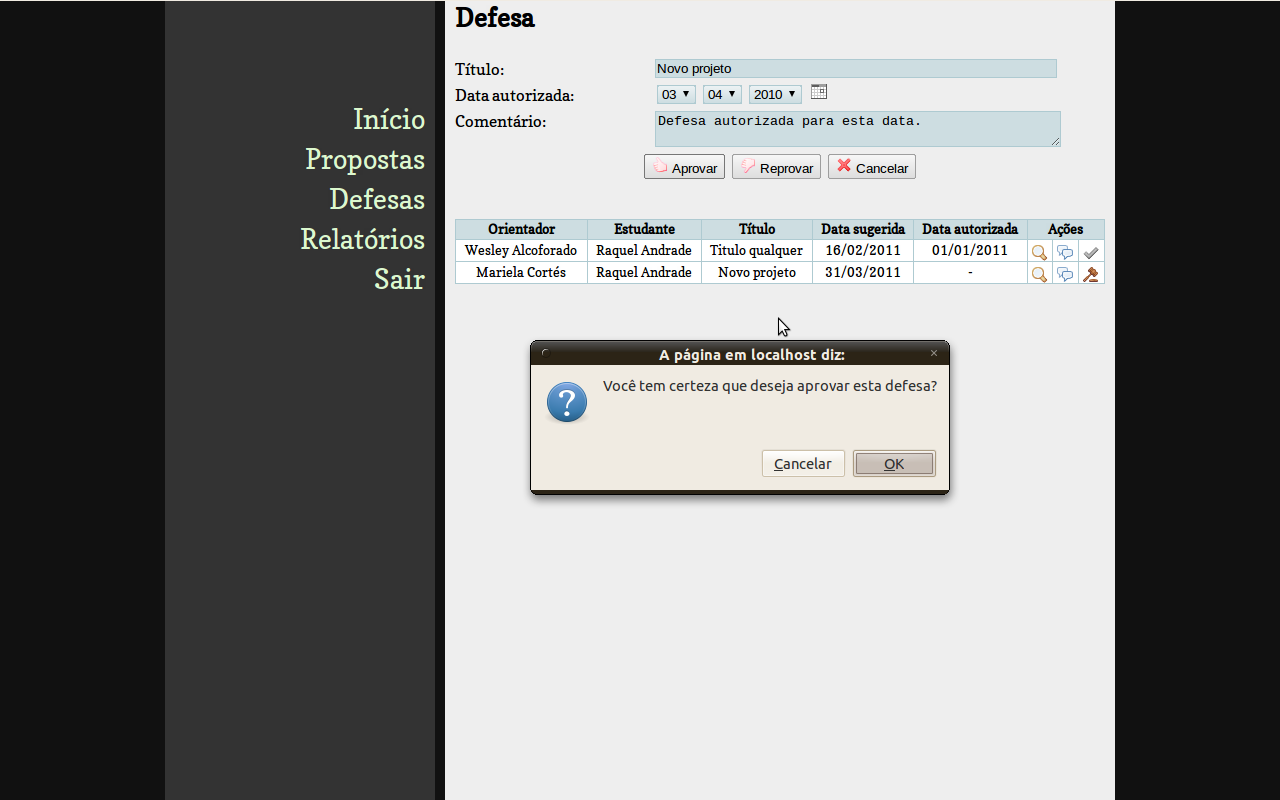
\includegraphics[width=1\textwidth]{fig/telas/processo/comissao_05_aprovando_defesa.png}
\caption{Tela de listagem de requisições de defesa no perfil da comissão}
\label{fig:comissao_05_aprovando_defesa}
\end{figure}

\begin{figure}[htbp]
\centering
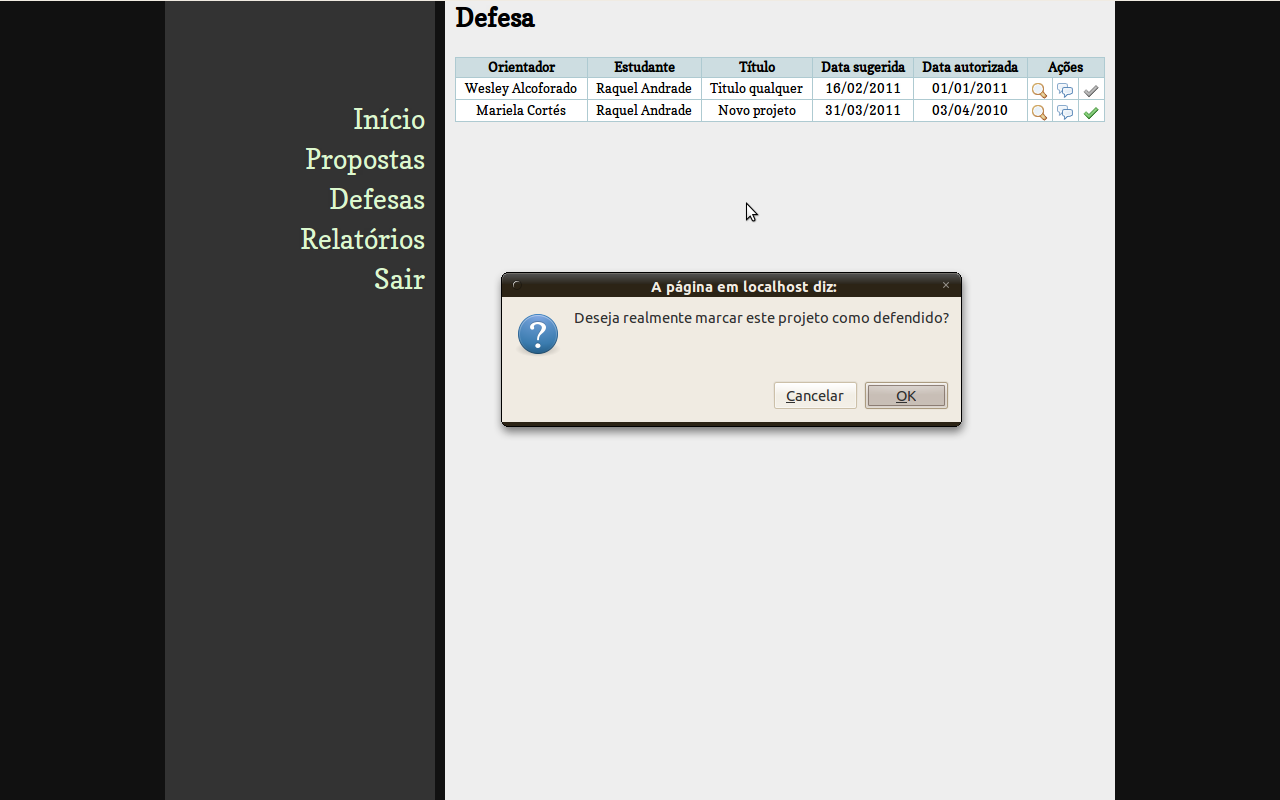
\includegraphics[width=1\textwidth]{fig/telas/processo/comissao_06_marcando_projeto_como_defendido.png}
\caption{Comissão marcando projeto como defendido}
\label{fig:comissao_06_marcando_projeto_como_defendido}
\end{figure}


\chapter{Conclusões e trabalhos futuros}
\label{cha:conclusoes}

Neste trabalho foi apresentada uma solução para um problema comum do dia-a-dia
da coordenação do curso de Ciências da Computação da UECE - ter que lidar com
muita papelada referente aos TCCs dos alunos.

A ferramenta se propõe a gerenciar o processo de submissão de projetos finais, seguindo
o regulamento estabelecido pela universidade, e também a manter todos atentos ao cumprimento
dos prazos.

Pessoalmente, espero que a aplicação desenvolvida neste trabalho seja útil
para o curso de Ciências da Computação da UECE, público alvo desta monografia, 
e que eu tenha conseguido dar minha humilde contribuição para o nosso curso,
de onde tirei a maior parte do meu conhecimento em computação.

\section{Trabalhos futuros}
A partir da contribuição apresentada pelo presente trabalho, alguns
trabalhos futuros podem ser indicados visando estender sua funcionalidade como:

\begin{itemize}
\item Construir um sistema de visualização e pesquisa das monografias defendidas, 
com exporta\-ção de citações para diferentes formatos, como o {\sc Bib}\TeX.
\item Estender o funcionamento do sistema para também atender defesas de mestrado e doutorado.
\item Generalizar a ferramenta para atender quaisquer tipo de defesa de qualquer curso universitário.
\end{itemize}


\bibliographystyle{abnt-alf}
\bibliography{bib}

%\appendix
\chapter{Apêndice}
\clearpage
\section{Casos de uso}
\subsection{Manter Professores}
\begin{longtable}{r p{12cm}}
\hline
Atores & Administrador \\ \hline
Pré-condições & O administrador deve estar logado no sistema.\\ \hline
Fluxo básico &1. O caso de uso se inicia quando o administrador seleciona manter professores no menu do sistema. \newline
                2. Uma vez que o administrador seleciona uma das opções disponíveis (incluir, alterar, excluir, listar): \newline
                \hspace*{1cm} a) Se o administrador selecionar a opção incluir, o caso de uso segue para o sub-fluxo 2 - Incluir Professor. \newline 
                \hspace*{1cm} b) Se o administrador selecionar a opção alterar, o caso de uso segue para o sub-fluxo 3 - Alterar Professor.  \newline 
                \hspace*{1cm} c) Se o administrador selecionar a opção excluir, o caso de uso segue para o sub-fluxo 4 - Excluir Professor.  \newline 
                \hspace*{1cm} d) Se o administrador selecionar a opção listar, o caso de uso segue para o sub-fluxo 5 - Listar Professores.  \newline 
                3. O caso de uso se encerra. \newline \\
Incluir Professor & 1. Este sub-fluxo se inicia quando o administrador seleciona incluir um novo professor. \newline
                    2. O sistema exibe os seguintes campos (os campos com asterisco são obrigatórios): \newline
                    \hspace*{1cm} * Nome de usuário \newline
                    \hspace*{1cm} * Email \newline
                    \hspace*{1cm} * Senha \newline
                    \hspace*{1cm} * Confirmação de senha \newline
                    \hspace*{1cm} Nome \newline
                    \hspace*{1cm} Sobrenome \newline
                    \hspace*{1cm} * Instituição \newline
                    \hspace*{1cm} * Titulação \newline
                    \hspace*{1cm} Experiência \newline
                    \hspace*{1cm} Substituto - Campo de escolha única fechada (valores: sim, não) \newline
                    \hspace*{1cm} Comissão - Campo de escolha única fechada (valores: sim, não) \newline
                    \hspace*{1cm} Ativo - Campo de escolha única fechada (valores: sim, não) \newline
                    \hspace*{1cm} Superusuário - Campo de escolha única fechada (valores: sim, não) \newline
                    3. O administrador preenche os campos e seleciona a opção salvar. \newline
                    4. O sistema valida se os campos obrigatórios foram preenchidos. \newline
                    5. O sistema inclui o professor no banco de dados. \newline
                    6. O caso de uso se encerra. \newline \\
Alterar Professor & Pré-condições: O administrador deve ter selecionado um professor para a alteração. \newline
                    1. Este sub-fluxo se inicia quando o administrador seleciona alterar professor.  \newline       
                    2. O sistema exibe os campos preenchidos.  \newline
                    3. O administrador altera os dados e solicita salvar os dados. \newline
                    4. O sistema valida se os campos obrigatórios foram preenchidos. \newline
                    5. O sistema salva as alterações no banco de dados. \newline
                    6. O caso de uso se encerra. \newline \\
Excluir Professor & Pré-condições: O administrador deve ter seleciona umdo professor para a exclusão. \newline
                    1. Este sub-fluxo se inicia quando o administrador seleciona excluir professor. \newline
                    2. O sistema solicita que o administrador confirme a exclusão. \newline
                    3. O adminstrador confirma a mensagem. \newline
                    4. O sistema exclui o professor do banco de dados. \newline
                    5. O caso de uso se encerra. \newline \\
Listar Professores & 1. Este sub-fluxo se inicia quando o administrador seleciona listar professores. \newline
                     2. O sistema exibe a listagem dos professores, contendo os seguintes campos:\newline
                     \hspace*{1cm} a) Nome\newline
                     \hspace*{1cm} b) Sobrenome\newline
                     \hspace*{1cm} c) Nome de usuário\newline
                     \hspace*{1cm} d) Email\newline
                     3. O caso de uso se encerra.               
               \\ \hline
Fluxos alternativos & Dados obrigatórios não preenchidos  \newline
                        1. Este sub-fluxo se inicia no passo 4 dos sub-fluxos Incluir Professor e Alterar Professor, quando o usuario não informou todos os campos obrigatórios. \newline
                        2. O sistema exibe ao lado do campo uma mensagem de que o campo deve ser preenchido e aguarda até que o administrador o preencha. \newline
                        3. O subfluxo segue para o passo 2 do sub-fluxo do qual ele se originou. 
                    \\ \hline        
\end{longtable}







\clearpage
\subsection{Manter Estudantes}
\begin{longtable}{r p{12cm}}
\hline
Atores & Administrador \\ \hline
Pré-condições & O administrador deve estar logado no sistema.\\
Fluxo básico & 1. O caso de uso se inicia quando o administrador seleciona manter estudantes no menu do sistema. \newline
                2. Uma vez que o administrador seleciona uma das opções disponíveis (incluir, alterar, excluir, listar): \newline
                \hspace*{1cm} a) Se o administrador selecionar a opção incluir, o caso de uso segue para o sub-fluxo 2 - Incluir Estudante. \newline 
                \hspace*{1cm} b) Se o administrador selecionar a opção alterar, o caso de uso segue para o sub-fluxo 3 - Alterar Estudante.  \newline 
                \hspace*{1cm} c) Se o administrador selecionar a opção excluir, o caso de uso segue para o sub-fluxo 4 - Excluir Estudante.  \newline 
                \hspace*{1cm} d) Se o administrador selecionar a opção listar, o caso de uso segue para o sub-fluxo 5 - Listar Estudantes.  \newline 
                3. O caso de uso se encerra. \newline \\
Incluir Estudante & 1. Este sub-fluxo se inicia quando o administrador seleciona incluir um novo estudante. \newline
                    2. O sistema exibe os seguintes campos (os campos com asterisco são obrigatórios): \newline
                    \hspace*{1cm} * Matrícula \newline
                    \hspace*{1cm} * Email \newline
                    \hspace*{1cm} * Senha \newline
                    \hspace*{1cm} * Confirmação de senha \newline
                    \hspace*{1cm} Nome \newline
                    \hspace*{1cm} Sobrenome \newline
                    \hspace*{1cm} Telefone \newline
                    \hspace*{1cm} Ativo - Campo de escolha única fechada (valores: sim, não) \newline
                    3. O administrador preenche os campos e seleciona a opção salvar. \newline
                    4. O sistema valida se os campos obrigatórios foram preenchidos. \newline
                    5. O sistema inclui o estudante no banco de dados. \newline
                    6. O caso de uso se encerra. \newline \\
Alterar Estudante & Pré-condições: O administrador deve ter selecionado um estudante para a alteração. \newline
                    1. Este sub-fluxo se inicia quando o administrador seleciona alterar estudante.  \newline       
                    2. O sistema exibe os campos preenchidos.  \newline
                    3. O administrador altera os dados e solicita salvar os dados. \newline
                    4. O sistema valida se os campos obrigatórios foram preenchidos. \newline
                    5. O sistema salva as alterações no banco de dados. \newline
                    6. O caso de uso se encerra. \newline \\
Excluir Estudante & Pré-condições: O administrador deve ter seleciona umdo estudante para a exclusão. \newline
                    1. Este sub-fluxo se inicia quando o administrador seleciona excluir estudante. \newline
                    2. O sistema solicita que o administrador confirme a exclusão. \newline
                    3. O adminstrador confirma a mensagem. \newline
                    4. O sistema exclui o estudante do banco de dados. \newline
                    5. O caso de uso se encerra. \newline \\
Listar Estudantes & 1. Este sub-fluxo se inicia quando o administrador seleciona listar estudantes. \newline
                     2. O sistema exibe a listagem dos estudantes, contendo os seguintes campos:\newline
                     \hspace*{1cm} a) Nome\newline
                     \hspace*{1cm} b) Sobrenome\newline
                     \hspace*{1cm} c) Matrícula\newline
                     \hspace*{1cm} d) Telefone\newline
                     \hspace*{1cm} e) Email\newline
                     3. O caso de uso se encerra.\newline                    
               \\ \hline
Fluxos alternativos & Dados obrigatórios não preenchidos  \newline
                        1. Este sub-fluxo se inicia no passo 4 dos sub-fluxos Incluir Estudante e Alterar Estudante, quando o usuario não informou todos os campos obrigatórios. \newline
                        2. O sistema exibe ao lado do campo uma mensagem de que o campo deve ser preenchido e aguarda até que o administrador o preencha. \newline
                        3. O subfluxo segue para o passo 2 do sub-fluxo do qual ele se originou. \newline
                    \\ \hline        
\end{longtable}







\clearpage
\subsection{Manter Projetos}
\begin{longtable}{r p{12cm}}
\hline
Atores & Estudante \\ \hline
Pré-condições & O estudante deve estar logado no sistema.\\ \hline
Fluxo básico &  1. O caso de uso se inicia quando o estudante seleciona manter projetos no menu do sistema. \newline
                2. Uma vez que o estudante seleciona uma das opções disponíveis (incluir, alterar, excluir, listar, visualizar comentários): \newline
                \hspace*{1cm} a) Se o estudante selecionar a opção incluir, o caso de uso segue para o sub-fluxo 2 - Incluir Projeto. \newline 
                \hspace*{1cm} b) Se o estudante selecionar a opção alterar, o caso de uso segue para o sub-fluxo 3 - Alterar Projeto.  \newline 
                \hspace*{1cm} c) Se o estudante selecionar a opção excluir, o caso de uso segue para o sub-fluxo 4 - Excluir Projeto.  \newline 
                \hspace*{1cm} d) Se o estudante selecionar a opção listar, o caso de uso segue para o sub-fluxo 5 - Listar Projetos.  \newline 
                \hspace*{1cm} e) Se o estudante selecionar a opção visualizar comentários, o caso de uso segue para o sub-fluxo 6 - Visualizar Comentarios.  \newline 
                3. O caso de uso se encerra. \newline \\
Incluir Projeto & 1. Este sub-fluxo se inicia quando o estudante seleciona incluir um novo projeto. \newline
                    2. O sistema exibe os seguintes campos (os campos com asterisco são obrigatórios): \newline
                    \hspace*{1cm} * Titulo \newline
                    \hspace*{1cm} * Orientador \newline
                    \hspace*{1cm} * Coorientadores \newline
                    3. O estudante preenche os campos e seleciona a opção salvar. \newline
                    4. O sistema valida se os campos obrigatórios foram preenchidos. \newline
                    5. O sistema inclui o projeto no banco de dados. \newline
                    6. O caso de uso se encerra. \newline \\
Alterar Projeto & Pré-condições: O estudante deve ter selecionado um projeto para a alteração. \newline
                    1. Este sub-fluxo se inicia quando o estudante seleciona alterar projeto.  \newline       
                    2. O sistema exibe os campos preenchidos.  \newline
                    3. O estudante altera os dados e solicita salvar os dados. \newline
                    4. O sistema valida se os campos obrigatórios foram preenchidos. \newline
                    5. O sistema salva as alterações no banco de dados. \newline
                    6. O caso de uso se encerra. \newline \\
Excluir Projeto & Pré-condições: O estudante deve ter selecionado um projeto para a exclusão. \newline
                    1. Este sub-fluxo se inicia quando o estudante seleciona excluir projeto. \newline
                    2. O sistema solicita que o projeto confirme a exclusão. \newline
                    3. O estudante confirma a mensagem. \newline
                    4. O sistema exclui o projeto do banco de dados. \newline
                    5. O caso de uso se encerra. \newline \\
Listar Projetos & 1. Este sub-fluxo se inicia quando o estudante seleciona listar projetos. \newline
                     2. O sistema exibe a listagem dos projetos, contendo os seguintes campos:\newline
                     \hspace*{1cm} a) Orientador\newline
                     \hspace*{1cm} b) Título\newline
                     \hspace*{1cm} c) Proposta\newline
                     \hspace*{1cm} d) Defesa\newline
                     \hspace*{1cm} e) Status - Status mais atual da defesa, ou se esta não tiver sido iniciada, o status mais atual da proposta.\newline
                     3. O caso de uso se encerra.\newline     \\ 
Visualizar Comentários & 1. Este sub-fluxo se inicia quando o estudante solicita visualizar os comentários. \newline
                     2. Uma vez que o estudante seleciona uma das opções disponíveis (comentários do orientador, da comissão):\newline
                     \hspace*{1cm} a) Se o estudante selecionar visualizar os comentários do orientador, o sistema exibe uma listagem com os comentários do orientador.\newline
                     \hspace*{1cm} b) Se o estudante selecionar visualizar os comentários da comissão, o sistema exibe uma listagem com os comentários da comissão.\newline
                     3. O caso de uso se encerra.                                        
               \\ \hline
Fluxos alternativos & Dados obrigatórios não preenchidos  \newline
                        1. Este sub-fluxo se inicia no passo 4 dos sub-fluxos Incluir Estudante e Alterar Estudante, quando o usuario não informou todos os campos obrigatórios. \newline
                        2. O sistema exibe ao lado do campo uma mensagem de que o campo deve ser preenchido e aguarda até que o administrador o preencha. \newline
                        3. O subfluxo segue para o passo 2 do sub-fluxo do qual ele se originou. 
                    \\ \hline        
\end{longtable}







\clearpage
\subsection{Manter Propostas}
\begin{longtable}{r p{12cm}}
\hline
Atores & Estudante, Orientador, Comissão \\ \hline
Pré-condições & O estudante deve estar logado no sistema e ter selecionado um projeto.\newline
                O orientador deve estar logado no sistema.\newline
                A comissão deve estar logada no sistema. \\ \hline
Fluxo básico &  1. O caso de uso se inicia quando o estudante seleciona a opção Anexar Proposta para o projeto selecionado. \newline
                2. O sistema exibe o campo Documento \newline
                3. O estudante escolhe um arquivo PDF e seleciona a opção Salvar. \newline
                4. O sistema valida o formato e tamanho do arquivo. \newline
                5. O sistema anexa o documento ao projeto, exibe uma mensagem de sucesso e redireciona o estudante à listagem de projetos. \newline
                6. O sistema envia um email ao orientador, informando do envio de uma nova proposta por um de seus orientandos.  \newline
                7. O orientador seleciona a opção Visualiza Proposta, do projeto em questão. \newline
                8. O sistema exibe a proposta e solicita ao orientador para que ele seleciona uma das opções disponíveis (Aprovar/desaprovar) \newline
                9. O orientador seleciona a opção aprovar.   \newline
                10. O sistema envia um email à comissão, informando do envio de uma nova proposta e atualiza o status da proposta para "Aprovada pelo orientador". \newline
                11. A comissão seleciona a opção Visualizar Proposta, do projeto em questão. \newline
                12. O sistema exibe a proposta e um campo de comentários e solicita à comissão para que ela selecione uma das opções disponíveis (Aprovar/desaprovar) \newline
                13. A comissão comenta (opcionalmente) na proposta e a aprova. \newline
                14. O sistema envia um email ao orientador e ao estudante, informando de que a proposta foi aprovada e atualiza o status da proposta para "Aprovada pela comissão". \newline
                15. O caso de uso se encerra.    \newline
               \\ \hline
Fluxos alternativos & Formato e/ou tamanho inválidos \newline
                        1. O subfluxo se inicia no passo 4 do fluxo básico, quando o sistema detecta que o formato e/ou o tamanho do arquivo são inválidos. \newline
                        2. O sistema informa ao usuário dos dados inválidos e solicita-o que os corrija. \newline
                        3. O subfluxo segue para o passo 2 do fluxo básico. \newline
                    
                    Desaprovação da proposta \newline
                        1. O subfluxo se inicia no passo 9 do fluxo básico, quando o usuário for o orientador, ou no passo 13 do fluxo básico, quando o usuário for da comissão. O usuário selecionou a reprovar. \newline
                        2. O sistema envia um email ao estudante (e ao orientador, caso a proposta tenha sido reprovada pela comissão), informando que sua proposta foi reprovada. \newline
                        3. O sistema atualiza o status da proposta para "Reprovada pelo orientador" ou "Reprovada pela comissão", dependendo de qual usuário tenha reprovado a proposta. \newline
                        4. O caso de uso se encerra. \newline
                    \\ \hline        
\end{longtable}







\clearpage
\subsection{Manter Defesas}
\begin{longtable}{r p{12cm}}
\hline
Atores & Estudante, Orientador, Comissão \\ \hline
Pré-condições & O estudante deve estar logado no sistema e ter selecionado um projeto.\newline
                O orientador deve estar logado no sistema.\newline
                A comissão deve estar logada no sistema. \\ \hline
Fluxo básico &  1. O caso de uso se inicia quando o estudante seleciona a opção Solicitar Defesa para o projeto selecionado. \newline
                2. O sistema exibe os seguintes campos: \newline
                \hspace*{1cm} a) Quantidade de páginas da monografia \newline 
                \hspace*{1cm} b) Data sugerida para realização da defesa  \newline 
                \hspace*{1cm} c) Copião (arquivo PDF)  \newline 
                3. O estudante preenche os campos e seleciona a opção Salvar. \newline
                4. O sistema valida os campos. \newline
                5. O sistema anexa o copião ao projeto, exibe uma mensagem de sucesso e redireciona o estudante à listagem de projetos. \newline
                6. O sistema envia um email ao orientador, informando do envio da solicitação de defesa por um de seus orientandos.   \newline
                7. O orientador seleciona a opção Solicitação de Defesa, do projeto em questão. \newline
                8. O sistema exibe o copião e solicita ao orientador para que ele selecione uma das opções disponíveis (Aprovar/desaprovar) \newline
                9. O orientador seleciona a opção aprovar.   \newline
                10. O sistema envia um email à comissão, informando do envio de uma nova solicitação de defesa e atualiza o status do projeto para "Defesa aprovada pelo orientador". \newline
                11. A comissão seleciona a opção Solicitação de Defesa, do projeto em questão. \newline
                12. O sistema exibe os seguintes campos: \newline
                    \hspace*{1cm} a) Copião (arquivo para download) \newline 
                    \hspace*{1cm} b) Comentários \newline 
                    \hspace*{1cm} c) Data autorizada para realização da defesa \newline
                13. O sistema solicita à comissão para que ela selecione uma das opções disponíveis (Aprovar/Desaprovar) \newline
                14. A comissão comenta (opcionalmente) na solicitação, preenche a data de realização da defesa e a aprova. \newline
                15. O sistema envia um email ao orientador e ao estudante, informando de que a solicitação foi aprovada e atualiza o status do projeto para "Defesa aprovada pela comissão".    \newline
                16. O caso de uso se encerra. 
               \\ \hline
Fluxos alternativos & Formato e/ou tamanho inválidos \newline
                        1. O subfluxo se inicia no passo 4 do fluxo básico, quando o sistema detecta que o formato e/ou o tamanho do arquivo são inválidos. \newline
                        2. O sistema informa ao usuário dos dados inválidos e solicita-o que os corrija. \newline
                        3. O subfluxo segue para o passo 2 do fluxo básico. \newline
                    
                    Desaprovação da proposta \newline
                        1. O subfluxo se inicia no passo 9 do fluxo básico, quando o usuário for o orientador, ou no passo 13 do fluxo básico, quando o usuário for da comissão. O usuário selecionou a reprovar. \newline
                        2. O sistema envia um email ao estudante (e ao orientador, caso a proposta tenha sido reprovada pela comissão), informando que sua proposta foi reprovada. \newline
                        3. O sistema atualiza o status da proposta para "Reprovada pelo orientador" ou "Reprovada pela comissão", dependendo de qual usuário tenha reprovado a proposta. \newline
                        4. O caso de uso se encerra. 
                    \\ \hline        
\end{longtable}








\chapter{Anexos}
\clearpage
\section{Formulário de proposta de projeto final}
\label{anx:proposta}
\begin{figure}[htbp]
\centering
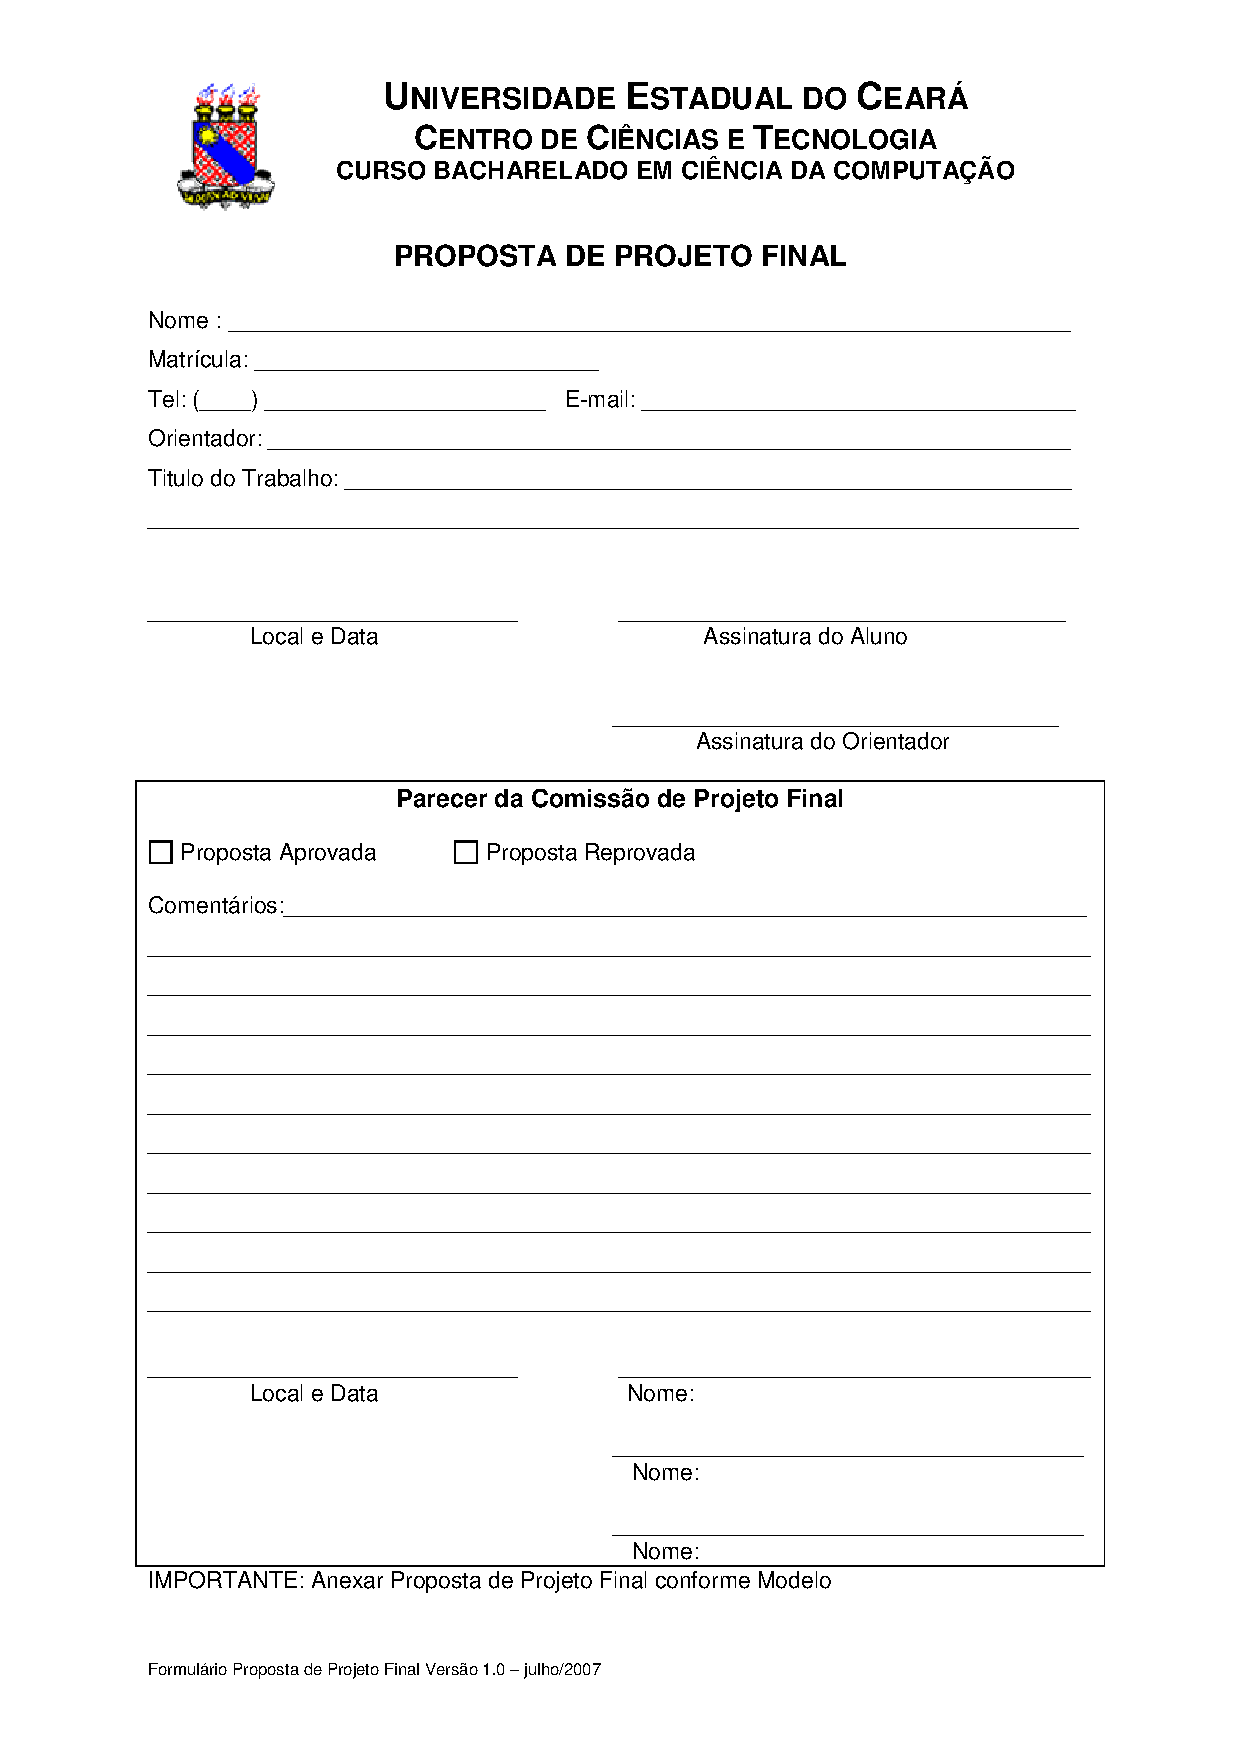
\includegraphics[scale=0.6]{requisitos/Formulario_Proposta_Projeto_Final.pdf}
\end{figure}

\clearpage
\section{Formulário de solicitação de defesa e banca}
\label{anx:defesa}
\begin{figure}[htbp]
\centering
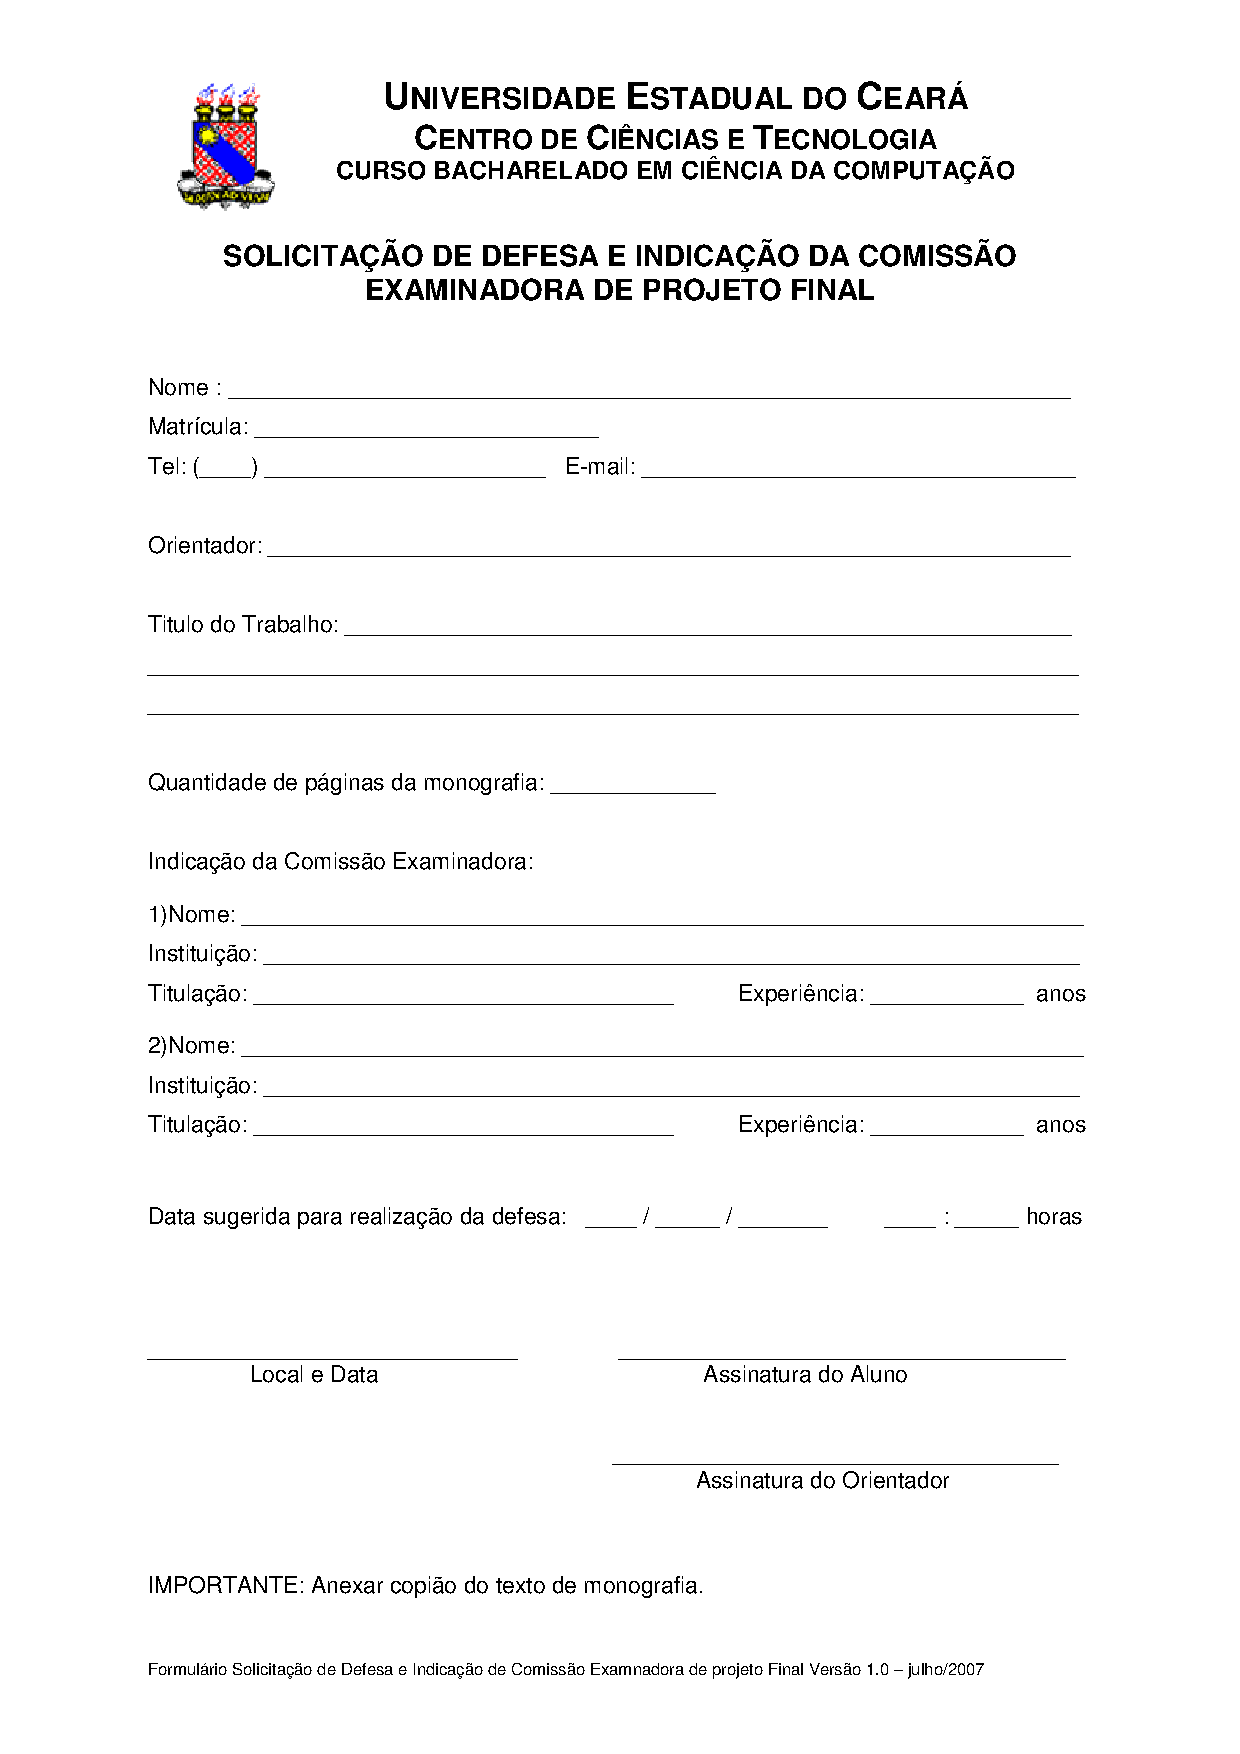
\includegraphics[scale=0.6]{requisitos/Formulario_Solicitacao_Defesa_e_Banca_v1.pdf}
\end{figure}



\end{document}

